\documentclass[12pt, a4paper, twoside, pdftex]{scrbook}

% Generelles
\usepackage[utf8]{inputenc}
\usepackage[main=english]{babel}
\usepackage{setspace}
\usepackage{hyperref}
\usepackage{array}
\hypersetup{
    colorlinks,
    citecolor=black,
    filecolor=black,
    linkcolor=black,
    urlcolor=black
}
\usepackage[a4paper, left=1.5cm, right=3.0cm, bottom=3.5cm]{geometry}
\usepackage{float}

% Images
\usepackage{graphicx}
\usepackage[export]{adjustbox}
\usepackage{tikz}

% Literatur
\usepackage[backend=biber,style=numeric]{biblatex}
\usepackage{csquotes}


\addbibresource{library.bib} %Imports bibliography file

\titlehead{
    \begin{tikzpicture}[remember picture,overlay]
        \node[anchor=north east,inner sep=0.5cm] at (current page.north east)
            {
            
\includegraphics[scale=0.5]{pictures/general/fh-muenster-logo}
            
\includegraphics[scale=0.2]{pictures/general/kubermatic-stacked}
        };
    \end{tikzpicture}
}

\title{\huge \textbf Design and implementation of a multi cluster load balancing within a Kubernetes environment}
\subtitle{Bachelor thesis to obtain the academic degree Bachelor of Science in Computer Science}
\author{Matthias Osthues\\
Department of Electrical Engineering and Computer Science\\
Fachhochschule Münster\\
University of Applied Sciences}
\publishers{
    \begin{flushleft}
        \small
        	\begin{onehalfspace}
        \begin{tabular}{l@{\hspace{1.0cm}} l}
            & \\
            & \\
            & \\
            & \\
            & \\
            & \\
            & \\
            & \\
            & \\
            & \\
            & \\
            First examiner	 	& Prof. Dr. Michael Tüxen \\
            Second examiner 	& Dipl.-Inf. Sebastian Scheele\\
            &\\
            submitted on	    & xx.xx.2021 \\
            from			    & Matthias Osthues \\
            Matriculation-Nr.   & 776405
        \end{tabular}
        	\end{onehalfspace}
    \end{flushleft}
}
\date{xx.xx.2021}
\begin{document}
    \maketitle

    \newpage
    \clearpage
    \tableofcontents
    \newpage

    \begin{onehalfspacing}

        \chapter{Introduction}


\section{Motivation and goal}
%Cloud computing
With the advent of cloud computing platforms such as AWS, GCP or Azure, the supply of dynamically scalable compute resources has changed.
To ensure the scalability of an application, this can be used to dynamically create new resources in case of a large load on the existing systems.
This requires a dynamic environment in which new servers can be automatically integrated into the existing infrastructure.
Among other things, network configurations and server provisioning must be ensured.
However, classical systems are often not built to scale across multiple hosts and must be reinvented or adapted accordingly.
\\
%cloud native
To simplify the complexity of managing compute resources, as well as deploying and scaling an application, so-called container orchestration systems were built with the advent of Docker.
One of these systems, which has found great acceptance in the market, is Kubernetes.
It follows the cloud-native\footnote{https://github.com/cncf/toc/blob/main/DEFINITION.md} approach, which is due to a constantly changing environment.
In the following, the terms CLuster refers to a Kubernetes cluster and nodes are the number of servers that are grouped together in a cluster.
In the event of a crash or the removal or addition of a node, Kubernetes ensures that the application can continue to run.
With Kubernetes, it is therefore comparatively easy to distribute an application across multiple servers and ensure scalability.
\\
%Load Balancers in cloud native
With the potentially ever-changing number of nodes, the question of load balancing also arises.
Typically, load balancers are used to serve as entry points and distribute traffic across multiple servers.
In a cloud-native environment, the configuration of a load balancer must also adapt to the constantly changing environment.
\\
Kubernetes provides a basis for dynamically creating/deleting and adapting an external load balancer.
However, it does not offer an out-of-the-box implementation of load balancers for clusters.
The implementations of load balancer is only available at various IaaS platforms (GCP, AWS, Azure).
This means for bare-metal clusters a manual integration for a load balancer service.
\\
%KKP
Kubermatic GmbH sells the Kubermatic Kubernetes Platform\footnote{https://www.kubermatic.com/products/kubermatic/}, which extends the cloud-native approach to Kubernetes clusters.
The platform can be used to dynamically create, delete and modify clusters.
With the advent of large scale deployments with multiple clusters, there is a need for a centralized load balancing solution for dynamically created clusters in a bare metal environment.
There are several solutions for implementing load balancers, but these are designed for one cluster and usually require their own network setup.
The Project KubeLB\footnote{https://github.com/kubermatic/kubelb} aims to provide a load balancer integration for multiple clusters and takes the advantages of kubernetes itself.

\newpage

\section{Structure of this work}
Following the introduction, the basics in the area of cloud-native and Kubernetes, as well as load balancing are first laid.

In the following chapter, the function of load balancers and the included network components and options with respect to Kubernetes will be discussed in more detail.

Chapter four discusses concepts and options within Kubernetes for extending functionality.

Subsequently, chapter five analyzes the concepts and transferability of the Kubermatic Kubernetes Platform and presents the KubeLB proposal.

In the sixth chapter, responsibility is distributed among subsystems, and a mechanism for communication between the individual components is described.
The interaction of the components is then modeled based on the underlying features of Layer 4 and Layer 7 load balancing.
Finally, the choice of the load balancer used is discussed.

Chapter seven describes the implementation of the components developed in chapter six and their integration into Kubernetes.

Following the implementation, software tests will be described.

The final chapter of the thesis draws a conclusion with regard to the technologies used, and the architectural design decisions.

This is followed in the last chapter by an outlook on further features that have not yet been implemented.


%\section{Cloud Native}
%Todo: add section
        \chapter{Basics}\label{basics}

This chapter provides a basic understanding of load balancing and Kubernetes.
The focus is mainly on the parts that are needed for the KubeLB Project.
It is not going into detail of everything and won't cover all load balancing features, algorithms and Kubernetes possibilities.
The load balancing part focuses on features that are commonly used inside a cloud environment, especially Kubernetes and is not covering other scenarios.

\section{Load Balancing}

A load balancer is a software or hardware device which distributes traffic among a set of servers.
They usually serve as an entrypoint and offer different features in a cloud environment.
\\
Load balancers offer a variety of algorithms for how traffic is distributed among endpoints:

\begin{itemize}\label{item:lb-algorithms}
    \item \textit{Random Load Balancing} \\
    As the name suggests, traffic is distributed randomly to the endpoints.
    This can result in one endpoint receiving a lot of traffic, and others receiving very little traffic.
    \item \textit{Round Robin} \\
    Traffic is sequentially forwarded to each endpoint.
    This method provides an evenly distributed amount of traffic to the endpoints.
    \item \textit{Weight Selection} \\
    The load balancer is told to send more traffic to the higher weighted endpoints than to others.
    \item \textit{Least Request} \\
    The load balancer tries to determine the endpoint with the least open requests.
    This highly depends on the load balancer implementation.
\end{itemize}

Choosing the best algorithm is not always trivial and depends on the application.~\cite{ALLEN-LOAD-BALANCING}
\\
For high available setups a load balancer can provide a failover mechanism.
This requires a health check mechanism, like Transmission Control Protocol (TCP) or Hypertext Transfer Protocol (HTTP) probes.
These probes are used to determine the endpoints healthiness and mark an endpoint as unhealthy if one or more probes fail.
When an endpoint becomes unhealthy, the load balancer stops forwarding traffic to it.
\\
Load balancers can operate on different levels of the Open Systems Interconnection model (OSI model).
Those are called layer 4 (Transport Layer) or layer 7 (Applikation layer) load balancers.
\\
A layer 4 load balancer takes place on the Transport layer, that means they are handling transport packets like TCP or UDP.
The fact that messages are neither inspected nor decrypted allows them to be forwarded quickly, efficiently, and securely.
\\
A layer 7 load balancer takes place on the Application layer, using protocols such as Hypertext Transfer Protocol and Stream Control Transmission Protocol (SCTP).
At this level the load balancer does have more information and can perform smarter decisions.
In terms of HTTP this means it can take routing decisions based upon HTTP Headers.
Transport Layer Security (TLS) termination is also handled by Layer 7 load balancers.~\cite{NICHOLSON-LOAD-BALANCING}

\section{Kubernetes}
``Kubernetes is an open-source container-orchestration system for automating computer application deployment, scaling, and management``\cite{Kubernetes}.
Kubernetes clusters contain a so called control-plane which is responsible for the cluster state.
The control-plane is a set of controllers which observe different objects of the cluster, react to change and trie to bring the cluster into it's desired state.
It also contains the information about the current cluster status.
\autoref{fig:kubernetes} gives an overview about the Kubernetes components.

\begin{figure}[H]
    \centering
    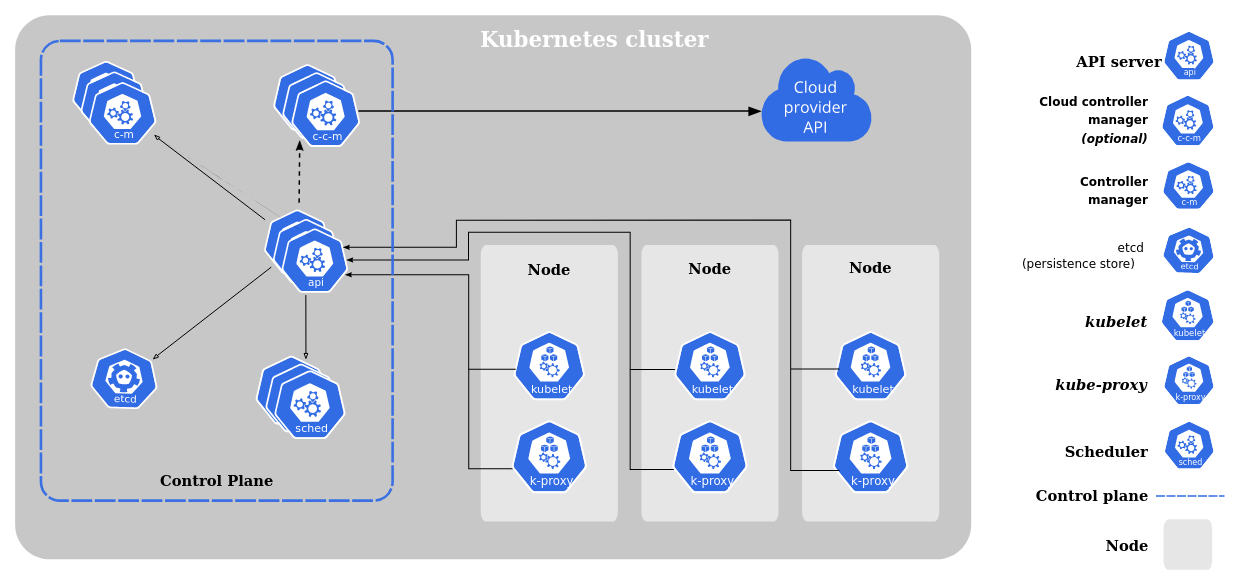
\includegraphics[width=1\linewidth]{media/02/kubernetes}
    \caption{"Components of Kubernetes" by The Linux Foundation CC BY 4.0}
    \label{fig:kubernetes}
\end{figure}

As \autoref{fig:kubernetes} shows, a node within the cluster consists of two components running on the host machine.

The kubelet daemon is responsible for the node status, and the containers that are deployed to it.
It serves like an agent to the cluster and communicates with the application programming interface (API) server.
Together with kubelet, the host needs an application that implements the Container Runtime Interface.\footnote{CRI: the Container Runtime Interface\footcite{CRI}}
This is required to run the actual container.
\\
Besides kubelet, kube-proxy is responsible for the networking part like routing and exposing services.
This is important for services to communicate inside the cluster.
A more detailed overview can be found in \autoref{sec:kubeproxy}.\cite{KUBERNETES-COMPONENTS}
\\
\newpage

Kubernetes offers a various set of building blocks ("primitives"), which describe different parts in the cluster to deploy an Application.
Each object shares the same basic data structure.

\begin{itemize}
    \item \textit{apiVersion} \\
    The API version to be used, either alpha, beta, or stable in different versions.
    \item \textit{kind} \\
    What kind is the object to create.
    \item \textit{metadata} \\
    Name, namespace and other metadata like labels and annotations.
    \item \textit{spec} \\
    The description of the state that is desired.
    The implementation differs for every object.
\end{itemize}

Some objects also have a status field that describes the current state.~\cite{KUBERNETES-OBJECTS}

\subsection{Pods}
A pod is a Kubernetes object, that describes a group of one or more containers.
Kubernetes manages pods instead of containers directly, so a pod is a wrapper around one or more containers.
It contains information of the docker image, volumes, ports and more.
An example of the information of a pod can be fond at \textit{spec.template} in \autoref{fig:deployment}.
The containers inside a pod share storage, network, and runtime specifications.
\\
There are applications where two containers are tightly coupled together.
Then it can make sense to deploy these containers together in one pod.
This ensures that the containers are deployed on the same node and have the same resources at their disposal, which has a positive effect on performance.
\\
A pod is not created directly, instead it is described inside a deployment, StatefulSet or DaemonSet.~\cite{KUBERNETES-POD}

\subsection{Deployment}\label{subsec:deployment}

A deployment takes track of the current state, make changes to an existing pods in a controlled rate, scaling and more.
It is widely used to deploy applications in a general purpose way.
The field \textit{spec.template} describes the actual pod created by the deployment, with its metadata and pod spec.
The \autoref{fig:deployment} illustrates an example deployment, with two containers and ports, inside a pod.
deployments have a selector which tells the controller which pod is controlled by this deployment.
The \textit{app: foo-bar} label is used as a selector and is also set within the template so that all pods created with this template are referenced to the deployment.
If applied, Kubernetes will create one pod, according to the replicas field, with two containers.
The containers use the same image, but with different environment variables and ports.
Those control what the HTTP service of the image will return and on what port it listens.~\cite{KUBERNETES-DEPLOYMENT}

\begin{figure}[H]
    \centering
    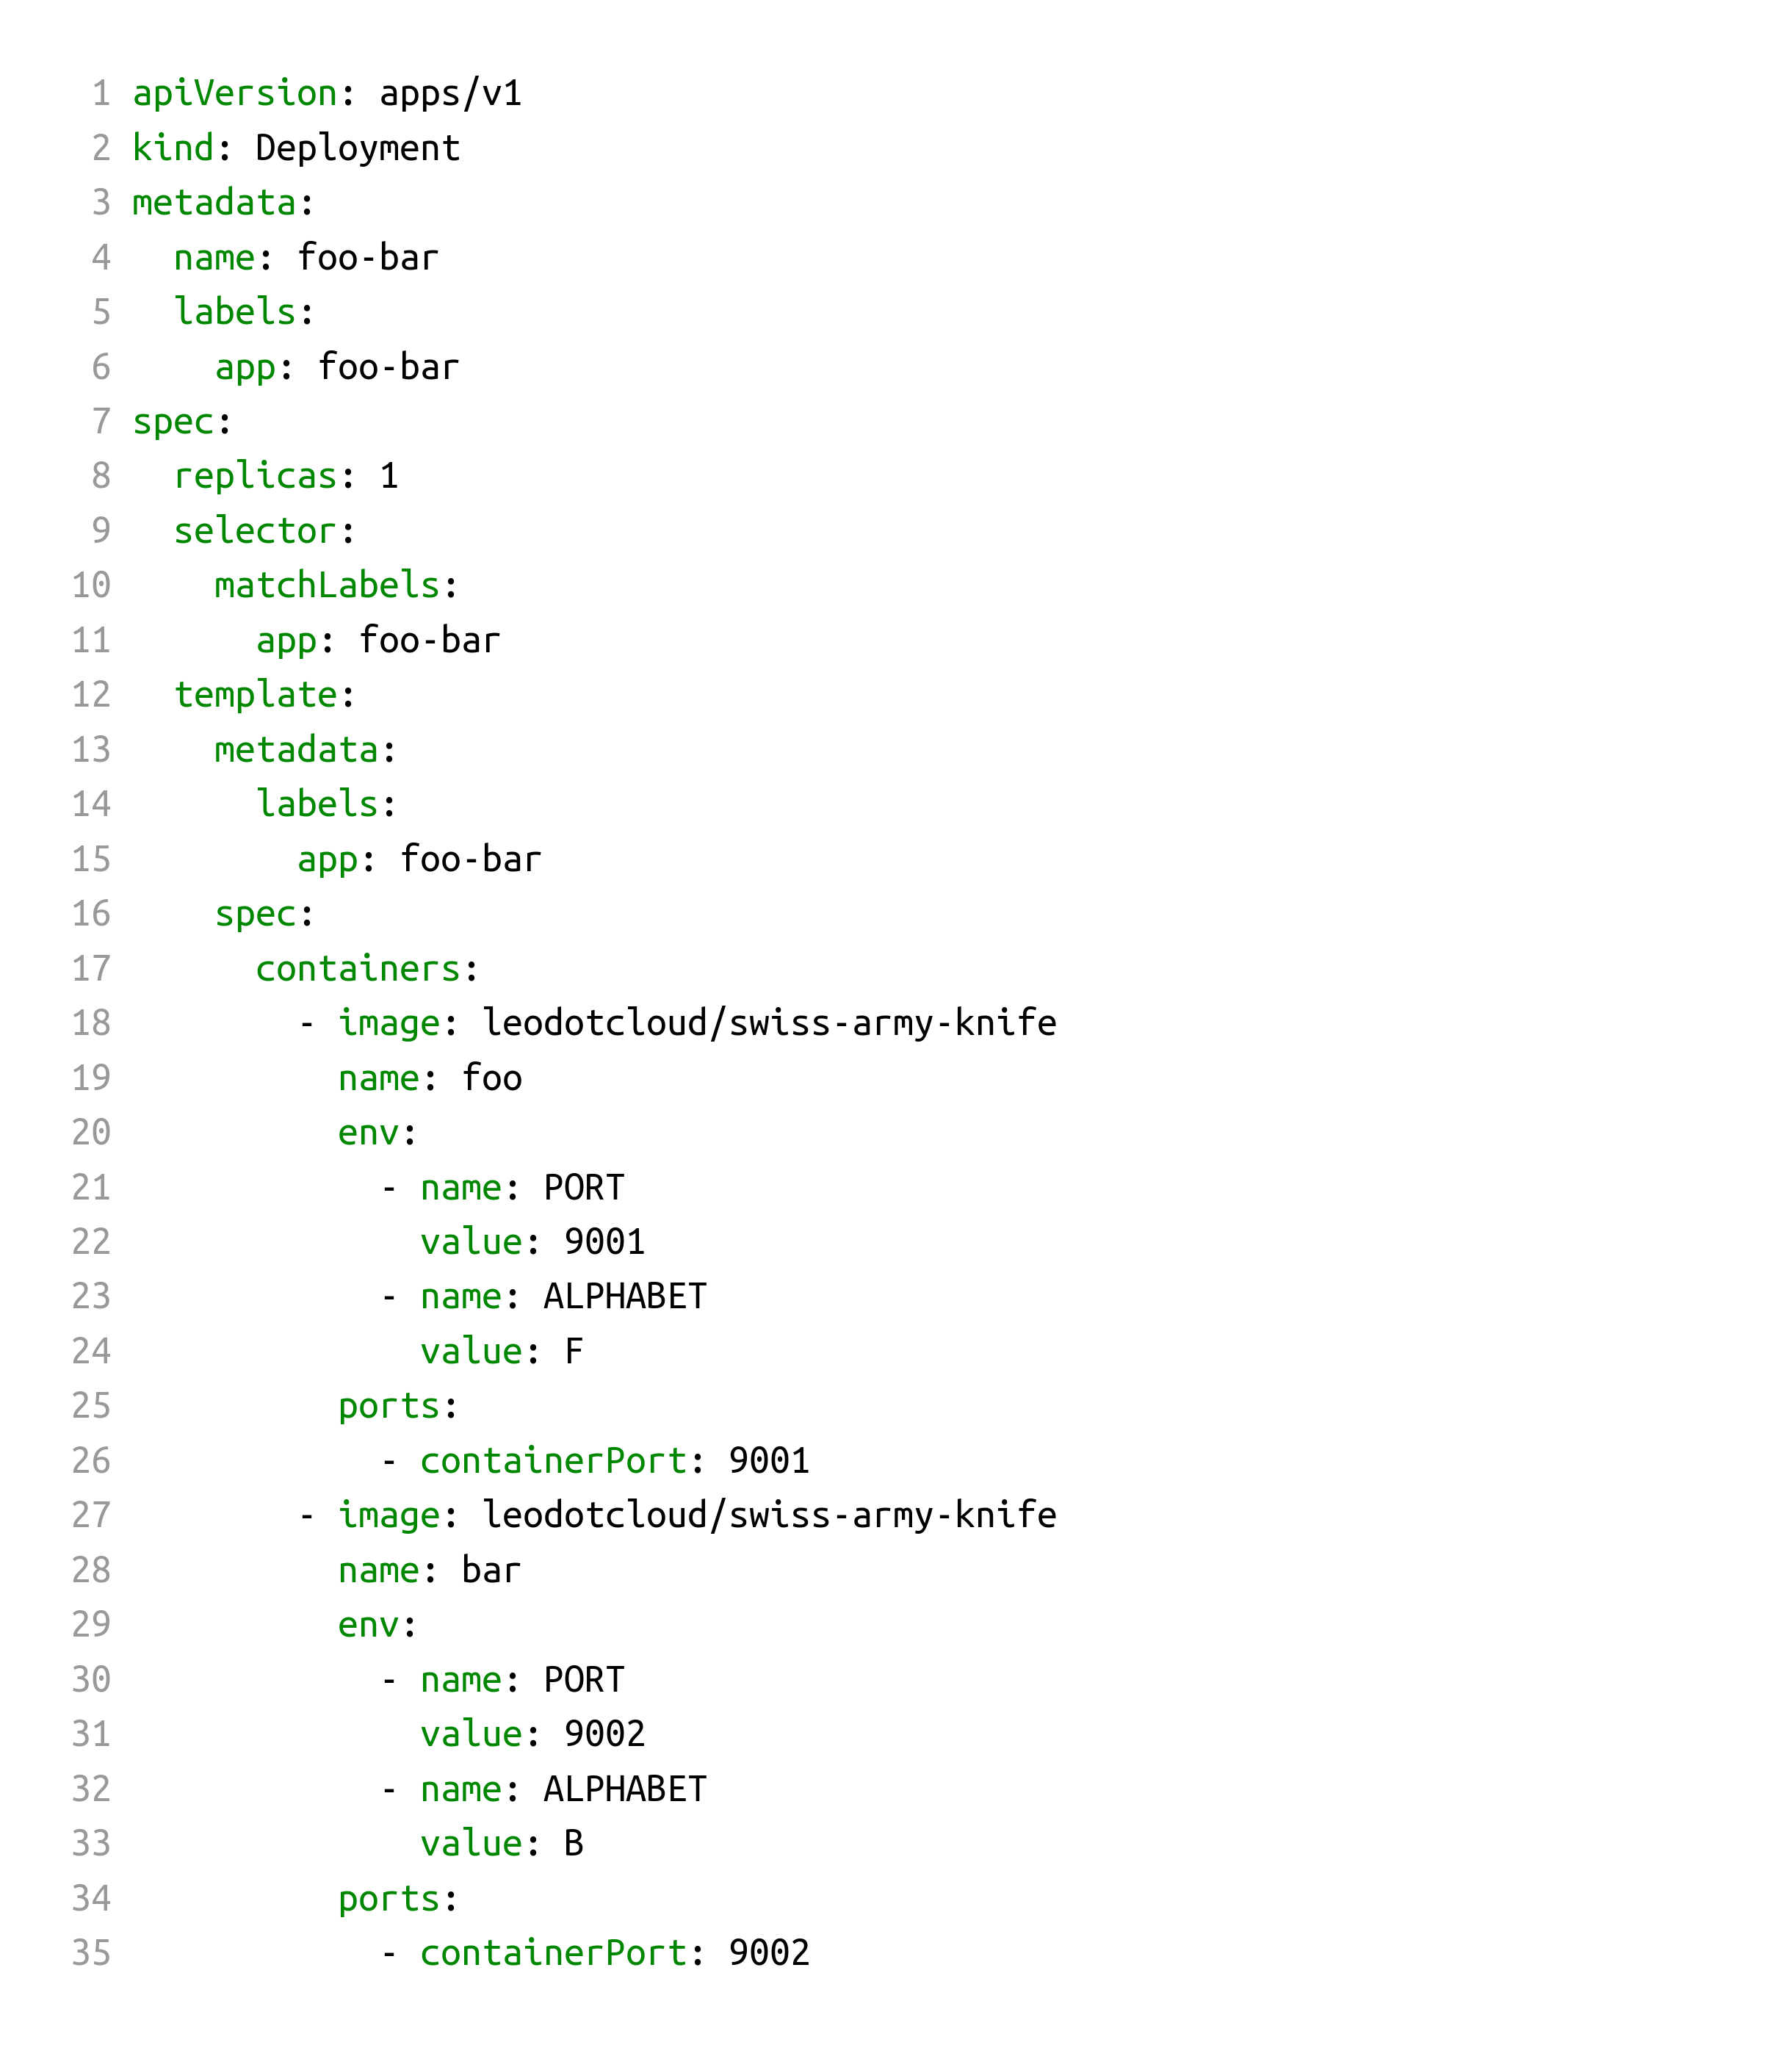
\includegraphics[width=0.8\textwidth, left]{media/02/deployment}
    \caption{Example deployment}
    \label{fig:deployment}
\end{figure}


\subsection{Service}\label{subsec:service}
To expose an application and make it accessible for others, the service object is used.
This is an abstraction of the networking layer and decides how to expose an application.
Services are used to open and map one or multiple ports of a pod.
The actual pod where the service applies to, is chosen by a selector.
This is important so that the controller knows to which pods the traffic is routed.
To keep track of which endpoints are currently available, the controller automatically creates an endpoint object.

\begin{figure}[H]
    \centering
    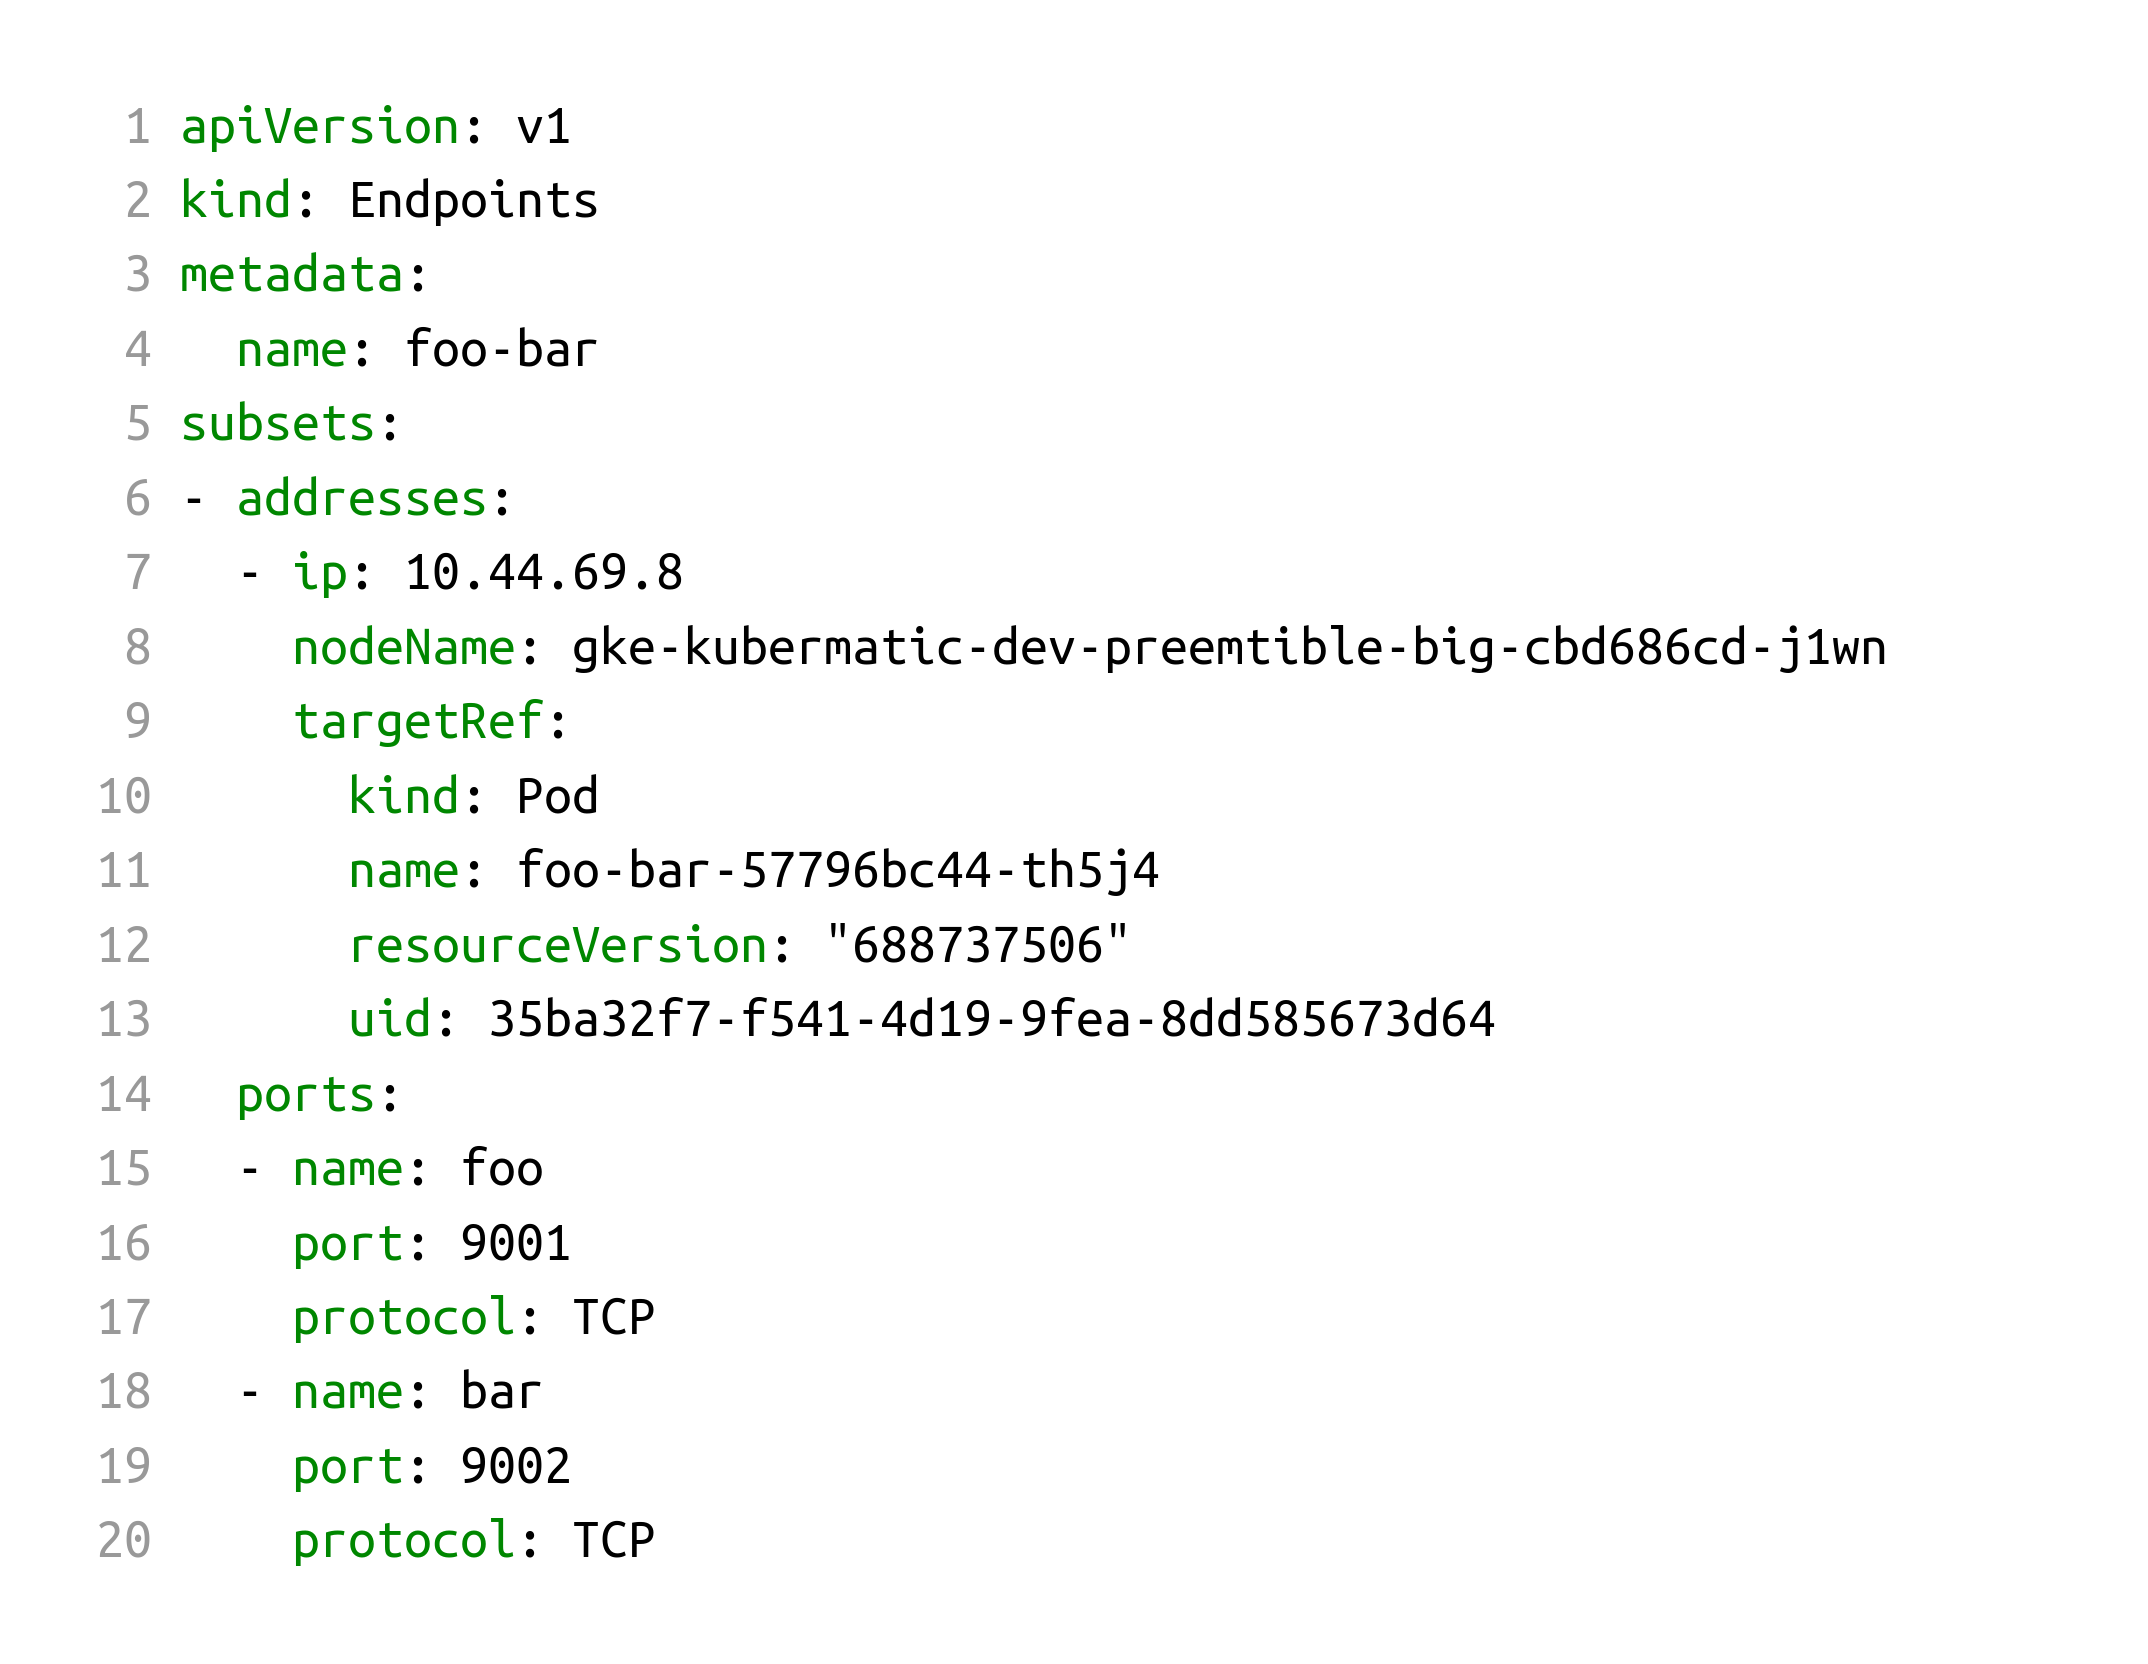
\includegraphics[width=0.8\textwidth, left]{media/02/endpoint}
    \caption{Example endpoints}
    \label{fig:endpoints}
\end{figure}

As \autoref{fig:endpoints} shows, an endpoint holds a list of IP addresses (in this case its just one as only one pod is deployed), as well as the associated ports.
In addition, the endpoints object is filled with further meta information by the controller.
Kubernetes scans for pods inside the cluster that match the given selector and updates the corresponding endpoint.
For a service without a selector, no associated endpoint is created and must be created otherwise.
TCP, UDP and SCTP are supported as protocols, TCP is the default.

\autoref{fig:service} shows an example service for the previous foo-bar deployment.
It exposes two ports one named foo at Port 8080, and bar at Port 8081.
Target port describes the Port of the actual pod and could be omitted because it is the same value as port, which describes the port to expose by the service.
The selector is \textit{app: foo-bar}, which was assigned to the pods as labels in the previous deployment.

\begin{figure}[H]
    \centering
    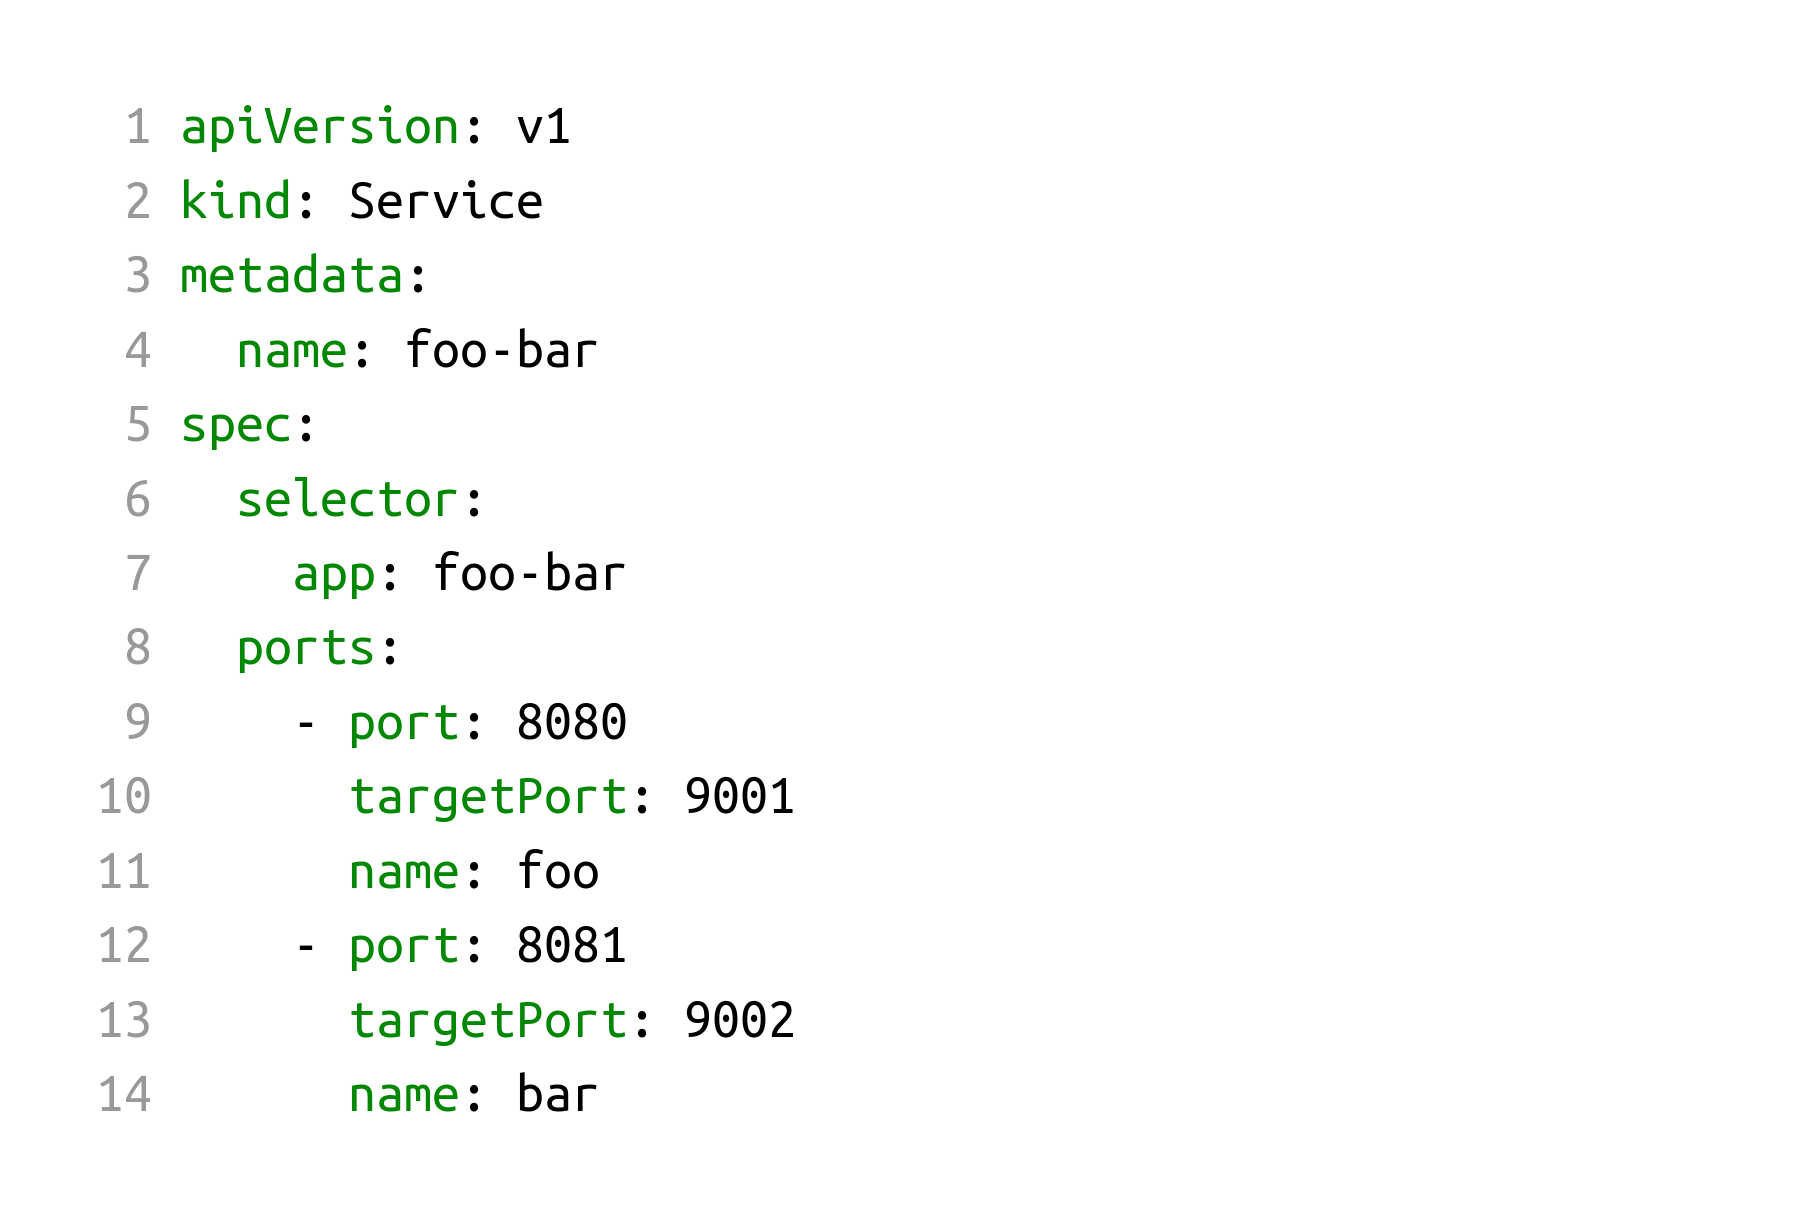
\includegraphics[width=0.7\textwidth, left]{media/02/service}
    \caption{Example service}
    \label{fig:service}
\end{figure}

It offers different types of exposing an application.
Type ClusterIp is the default and exposes the application only to other services inside the cluster.
These services can be addressed via an internal DNS.
Those DNS names follow by default this pattern: my-svc.my-namespace.svc.cluster-domain.example.
This is also the reason why the service name needs to be a valid DNS label.
\\
Type NodePort allocates a random port, by default in between of 30000-32767, and open this on all nodes of the cluster.
Thus, the service is externally accessible on all nodes of the cluster via the allocated port.
\\
Type LoadBalancer does the same as node port with the addition of an external implementation to dynamically create a load balancer and point it to the opened node ports.
This is not implemented by default and requires some extra setup for the cluster, what is explained in more detail in \autoref{sec:ExternalLoadBalancer}.~\cite{KUBERNETES-SERVICE}

\subsection{Ingress}\label{subsec:ingress}
The ingress is built as an addition to services and offers load balancing, TLS Termination or name-based virtual hosting.
Typically, it exposes only HTTP/HTTPS, other applications should make use of the service type NodePort or LoadBalancer.
It provides a number of configurable rules that decide to which backend the traffic is routed.
Thus, applications do not have to be directly exposed via a service, they only need to be internal accessible via ClusterIP.~\cite{KUBERNETES-INGRESS}
\autoref{fig:ingress} shows an example of an ingress object that forwards incoming HTTP requests with the /foo path to the foo-service on port 8080, and /bar path to the bar-service on port 8081.

\begin{figure}[H]
    \centering
    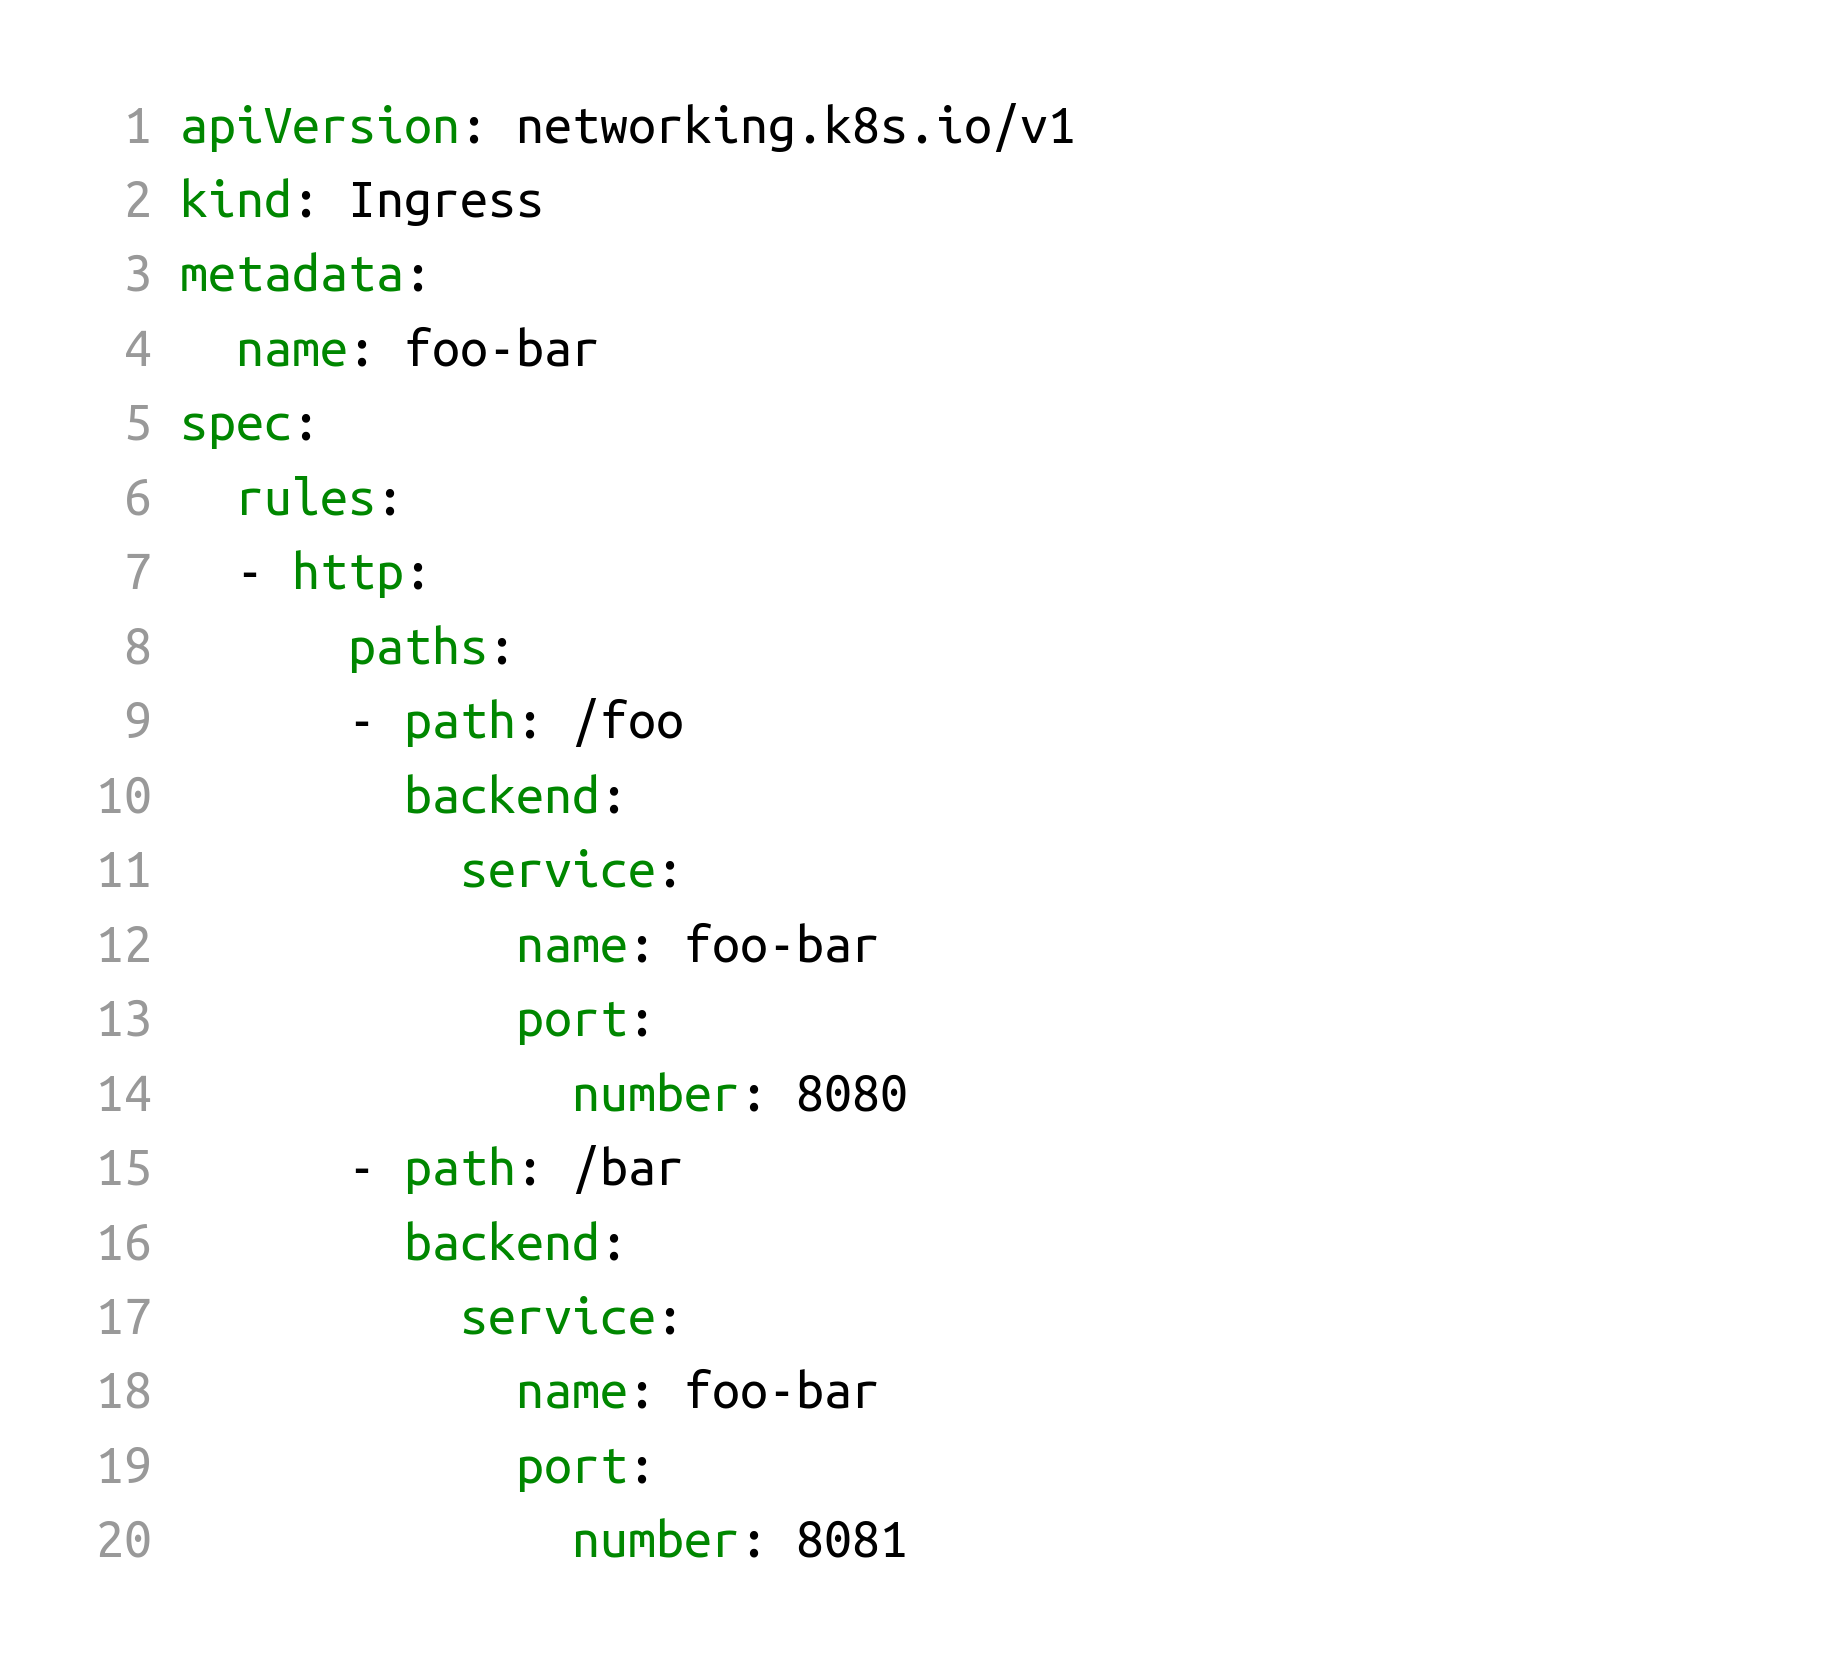
\includegraphics[width=0.7\textwidth, left]{media/02/ingress}
    \caption{Example ingress}
    \label{fig:ingress}
\end{figure}

To fulfill the ingress an IngressController must be installed.
The IngressController and its purpose will be explained in \autoref{sec:IngressController}.

        \chapter{Load Balancing with and for Kubernets}

\section{kube-proxy}\label{sec:kubeproxy}

\section{External Load Balancer}\label{sec:ExternalLoadBalancer}

\section{Ingress Controller}\label{sec:IngressController}

\section{Bare metal vs. cloud}

\section{KKP as a father}


        \chapter{Extending Kubernetes}

This chapter is about how to extend Kubernetes.
There are several ways to extend Kubernetes, this chapter focuses on Custom Resources and Controllers.

\section{Operator pattern}\label{sec:operator-pattern}

Operators are pieces of software that integrate in Kubernetes and manage applications.
The name originates from the fact that the software performs the tasks of a human operator.
The operator knows the system and knows how to deploy and configure it for different scenarios and at scale.~\cite{KUBERNETES-OPERATOR}
\\
A system administrator knows about the software, takes care of the deployment, monitoring and backups.
With the advent of the DevOps movement, this tradition has changed drastically.
The management of applications, monitoring, backups and entire cloud environments has been centralized and versioned using the Infrastructure as Code approach.
Through containers, the deployment of applications has also been standardized.
However, a system administrator is still required to react to state changes, that happen frequently inside a cloud native environment.
The operator therefore acts as a kind of robot sysadmin who can react directly to changes.~\cite{RED-HAT-OPERATOR}

\section{Custom Resource Definitions}\label{sec:custom-resource-definitions}

In Kubernetes \textit{Custom Resource Definitions}, in short CRDs, are used to extend the Kubernetes API.
A resource is a kubernetes API endpoint, like a Pod or Deployment.
These endpoints and data structures are predefined by Kubernetes.
A Custom Resource extends these with its own endpoint and data structure.
This allows data to be stored within the cluster.
Custom resources can be registered and de-registered at runtime.~\cite{KUBERNETES-CRD}

\section{Controllers}\label{sec:controllers}
A controller implements a control loop that constantly monitors the status of the cluster.
Depending on whether a certain change takes place, the controller reacts and makes adjustments where needed.
\\
The controller observes at least one Kubernetes resource.
The spec field within the resource represents the desired state.
Based on this, the controller tries to establish the desired state in the cluster.
In summary, the goal of a controller is to make the state of a cluster match the desired state.
\\
This is mostly done by calls to the Kubernetes API, but can also be reached by external API calls.
This is called direct control.
Since the state of external resources is not available within Kubernetes, such controllers usually use a status field, which is part of the Kubernetes resource, to reflect it in the cluster.
Other controllers can monitor this and then react in turn.
\\
To implement the Operator pattern, a custom controller is required.
~\cite{KUBERNETES-CONTROLLERS}
        \chapter{Requirements}

In diesem Kapitel werden die Rahmenbedingungen, welche bei Kubermatic vorhanden und für die Entwicklung der Anwendung relevant sind, untersucht.
Aus den Ergebnissen der Analyse sollen in einem zweiten Schritt Anforderungen an den zu entwickelnden Dienst abgeleitet werden.


\section{Kubermatic Kubernetes Platform}

``Kubermatic Kubernetes Platform (KKP) is in an open source project to centrally manage the global automation of thousands of Kubernetes clusters across multicloud, on-prem and edge with unparalleled density and resilience``~\cite{KKP-GITHUB}.

Due to the need of a central management solution for a multi cluster Kubernetes environment, KKP came up to solve this problem.
It aims to give the customer everything needed to build their own Kubernetes cloud environment. 
This includes a Multicloud Self Service Portal, HA Self-healing Infrastructure, Multi-tenancy and User Management, Monitoring and more.
A detailed list of the key features can be found on the Kubermatic website.\footnote{https://www.kubermatic.com/products/kubermatic/}
\\
To achieve resilience, KKP relies on Kubernetes itself.
This requires a so-called master cluster in which Kubermatic is installed, the master is the central instance in which all clusters are managed via KKP api.

\begin{figure}[H]
    \centering
    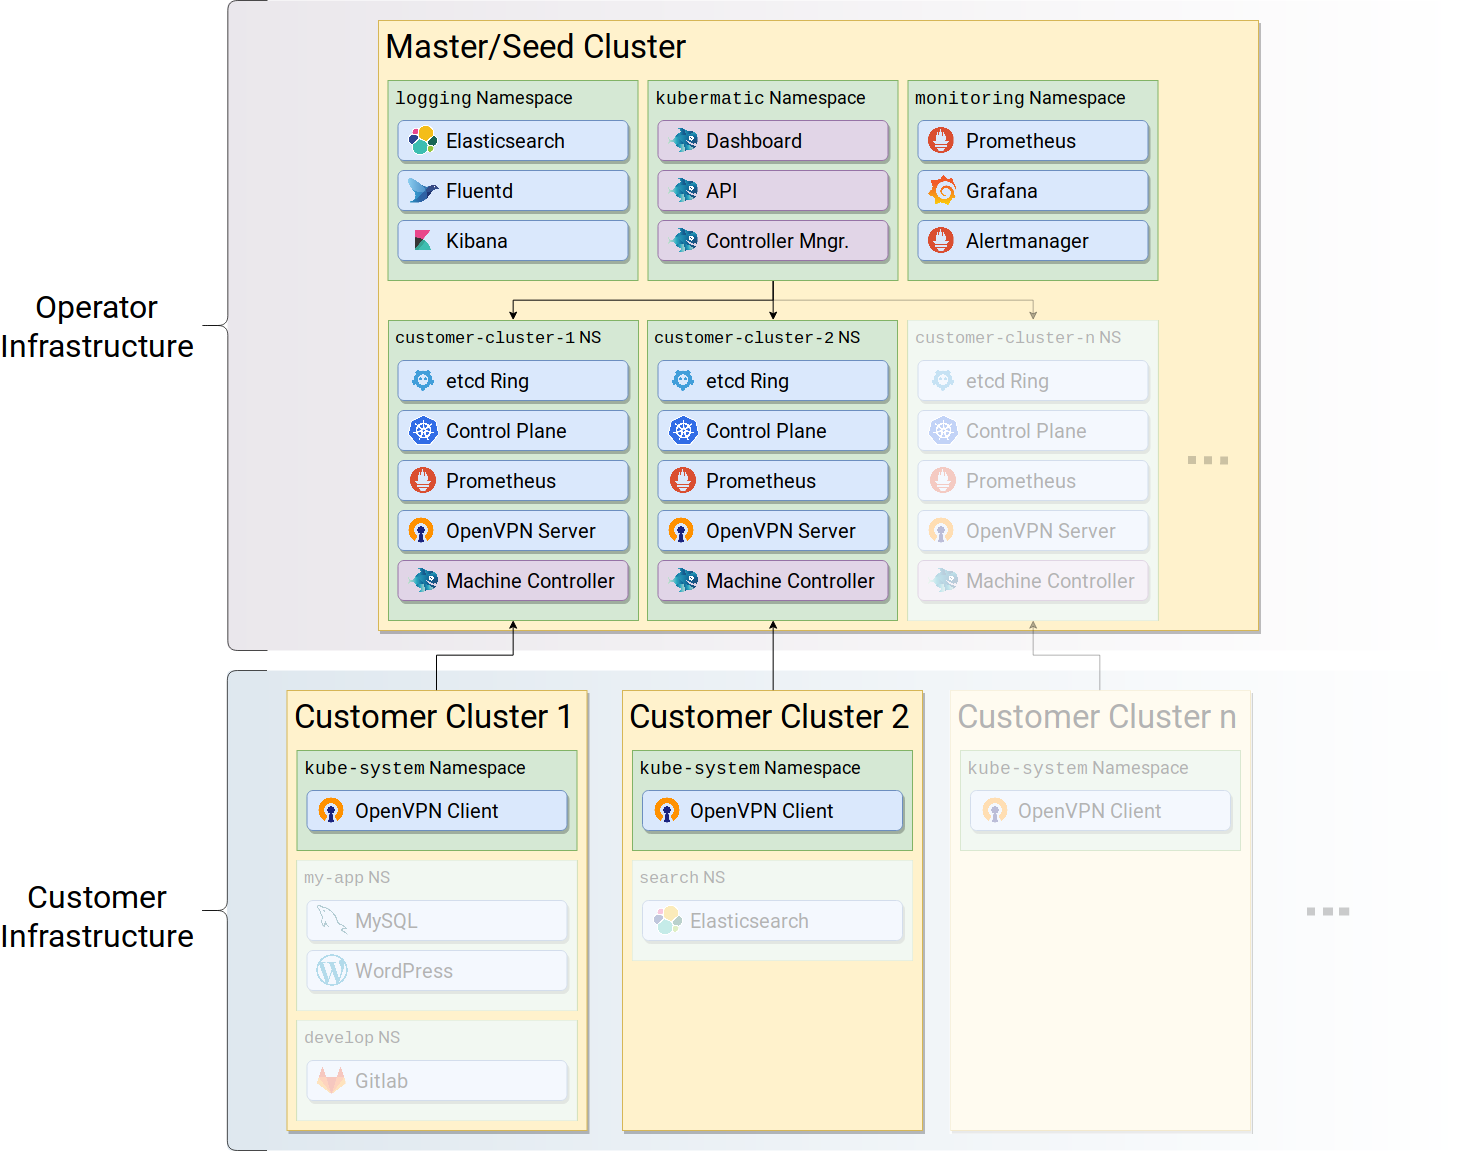
\includegraphics[width=1\textwidth, left]{media/05/kkp}
    \caption{"Kubermatic architecture, combined master seed" by Kubermatic GmbH CC BY 4.0}
    \label{fig:kubermatic}
\end{figure}

Another concept is the seed cluster, in which among other parts, the control-plane of a kubernetes cluster, that was created via KKP, lives.
As \autoref{fig:kubermatic} shows, the seed cluster can be the same as the master, but it is not mandatory.
Especially for large scale deployments it is recommended to run several independent seed clusters.
Thus, only worker nodes have to be created and connected.
Virtual machines are created via a supported provider, which are then provisioned by KKP and added as nodes.
\\
The master as well as the seed cluster should be operated in a high available setup.
This offers the advantage that the Kubernetes control plane of the customer cluster is automatically a High Available setup.


\section{KubeLB}\label{sec:KubeLB}

The idea behind KubeLB is to adopt concepts of KKP for load balancing in multicloud, on-prem and edge Kubernetes environments.
As mentioned in \autoref{sec:ExternalLoadBalancer}, load balancers need to be integrated manually to every cluster.
This is especially needed for bare metal environments, where no cloud provider solution is available.
The already existing open source solutions for the implementation of the load balancer, target single Kubernetes clusters, and are not designed for a highly dynamic multi cloud infrastructure.
\\
The main feature is the easy integration and availability of load balancing in many, dynamically created, Kubernetes clusters.
These clusters are referred to as \textit{user clusters} in the following.
For this purpose, a dedicated cluster is provided, which deploys a load balancer within the cluster, referred to as \textit{load balancer cluster} in the following.
In order to expose the load balancer in the cluster to the outside world, it is necessary for the load balancer cluster to have a load balancer implementation.
This has the advantage that load balancer integration only has to be performed once for the load balancer cluster, and simplifies the management of external IP addresses, as these can be managed centrally.
All features of the Kubernetes Service object of the load balancer type should be supported.
\\
In addition to the load balancer integration, layer 7 load balancing should also be offered.
This refers in particular to the Ingress resource and the ingress controller.
Since this, like the load balancer, is not automatically available within a Kubernetes cluster, integration should also be offered here.
For this purpose, a load balancer with Layer 7 properties, analogous to the Layer 4 load balancer, is to be deployed and made available within the load balancer cluster.
All features of the Kubernetes ingress object should be supported.
\\
To pass the requests for a load balancer or an ingress resource to the load balancer cluster, an Agent is provided within the user clusters.
The agent acts as a kind of cloud controller\footnote{https://kubernetes.io/docs/concepts/architecture/cloud-controller/}, which manages external resources of the cluster.
\\
In the cloud native community it is common to create a Proposal.
These should describe what the idea is, the goals being pursued, and include an architectural overview.
The original proposal can be found in the Kubermatic repository\footnote{https://github.com/kubermatic/kubermatic/blob/master/docs/proposals/kubelb.md} on github.

        \chapter{Design}

With the requirements discussed in \autoref{sec:KubeLB}, the next step is to design the architecture and determine the technologies to be used.
Since the core product of Kubermatic is based on Kubernetes, the KubeLB project also has to be operated in this context.
To adapt concepts from KKP, the goal is to use a Kubernetes cluster for load balancing.
This promotes a homogeneous environment of Kubernetes clusters without introducing additional complexity of third party systems, which simplifies both the deployment and the maintenance of the KubeLB application.

\section{Manager}\label{sec:manager}

The Manager, as already explained in \autoref{sec:operator-pattern}, will serve as an operator and implement a controller comparable to \autoref{sec:controllers}.
Its task is to observe a CRD~(see \autoref{sec:custom-resource-definitions}) and operate the load balancers within the load balancer cluster.
Those CRDs hold the desired configuration for the load balancers and are called TCPLoadBalancer for Layer 4, and HTTPLoadBalancer for Layer 7 load balancing.
\\
Within the load balancer cluster, different Kubernetes resources are used to reflect this.
The deployment~(see \autoref{subsec:deployment}) creates the actual load balancer within the cluster.
The service~(see \autoref{subsec:service}) exposes the load balancer deployment to the outside via a service of type LoadBalancer.
It should be noted that the load balancer cluster requires a load balancer implementation.
This can be either a cloud provider, or an Open Source single cluster implementation.
\\
Since the created service is of type LoadBalancer, the status field of the service gets updated with the external IP address.
The Manager should observe this and set the status field within the CRD.
\\
For layer 7 implementation, the Manager makes use of the ingress~(see \autoref{subsec:ingress}), therefore an ingress controller~(see \autoref{sec:IngressController}) must be installed as well.

\section{Agent}\label{sec:agent}

The Agent runs inside a user cluster and watches for services and ingress resources.
If needed, it creates a CRD with the details needed for the Manager inside the load balancer cluster.
Since the Agent runs inside the user cluster, it can read the desired configurations of the service or ingress resource and create, modify or delete the CRD appropriately.
\\
Likewise, it is able to get the endpoints and open ports for a service, that are required for the load balancer.
Since the cluster size, i.e.\ the number of nodes, can change dynamically, it is also the Agent's task to update the changed endpoints of the user cluster for all CRDs within the load balancer cluster.
\\
In the case of layer 4 load balancing, the Agent also sets the IP address in the status field of the service, which is set inside the status field of the CRD by the Manger.
\\
To interact with the load balancer cluster, the Agent needs access to a namespace to deploy the CRDs inside.

\section{Layer 4}

\autoref{fig:kubelb-l4} illustrates the architecture of layer 4 load balancing.
Within the user cluster, the Agent observes the service resource.
If a user creates a service of type LoadBalancer, the Agent recognizes the service and creates a TCPLoadBalancer inside the load balancer cluster.
\\
The Manager observes the TCPLoadBalancer CRD, which contains the necessary information to configure the load balancer.
Based on this, the Manager creates or updates the load balancer deployment and the associated service.


\begin{figure}[H]
    \centering
    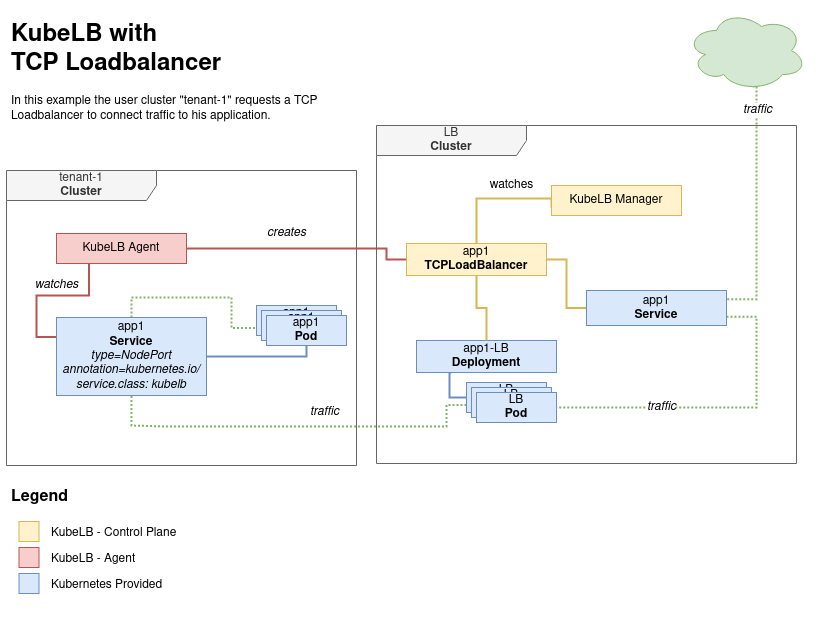
\includegraphics[width=1\linewidth]{media/06/kubelb-l4}
    \caption{"KubeLB Layer 4 architecture" by Kubermatic GmbH Apache License 2.0}
    \label{fig:kubelb-l4}
\end{figure}

\section{Layer 7}

Layer 7 load balancing introduces more complexity.
As \autoref{fig:kubelb-l7} shows, it relies on more components.
It is assumed that no ingress controller is installed inside the user cluster and KubeLB should fulfill the ingress, therefore some extra steps are required.
At first the service to expose via ingress could be of type ClusterIP, in this case it is not reachable for the load balancer inside the load balancer cluster.
In this case the Agent copies the existing service and creates a new one of type node port, so it is actually exposed and accessible to the load balancer.
\\
The second part is to create a TCPLoadBalancer, based on the copied service, inside the load balancer cluster.
Since KubeLB makes use of the ingress controller implementation, it needs some kind of connector to the user cluster.
Ingress is, by design, cluster based and only routable to internal services.
For that reason it is mandatory to have an internal load balancer service, accessible for the ingress controller.
It is not necessary to expose the load balancer, so the Agent sets the service type inside the TCPLoadBalancer to ClusterIP.
\\
At this point the Agent creates a HTTPLoadBalancer, based on the ingress inside the user cluster, inside the load balancer cluster.
The Manager takes care that the ingress is configured to use the corresponding load balancer service, which was created before.

\begin{figure}[H]
    \centering
    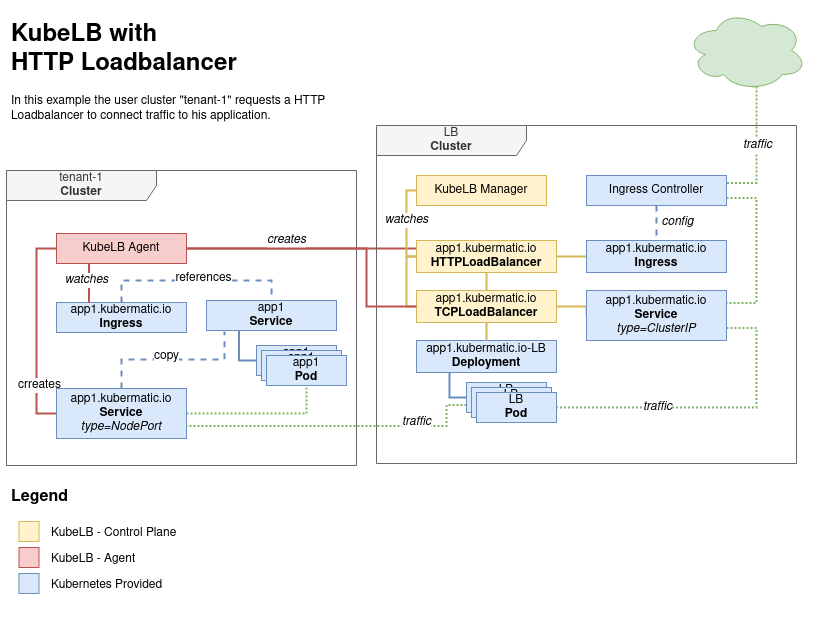
\includegraphics[width=1\linewidth]{media/06/kubelb-l7}
    \caption{"KubeLB Layer 7 architecture" by Kubermatic GmbH Apache License 2.0}
    \label{fig:kubelb-l7}
\end{figure}

\section{Envoy}\label{sec:envoy}

Envoy is chosen as a load balancer instance because of its design for large modern service oriented architectures and its high feature set.
Nginx and HA-Proxy offer similar functionalities, but are not initially developed for the required purposes inside a cloud native environment.
\\
The most important functions needed for KubeLB are summarized below:

\begin{itemize}
    \item \textit{L3/L4 filter architecture} \\
    The Envoy core is a L3/L4 network proxy, that is configurable via filter chains, allowing the proxy to perform different TCP/UDP tasks.
    \item \textit{HTTP L7 filter architecture} \\
    Since HTTP is widely used for applications to communicate, envoy offers an additional Layer 7 filter architecture on top, which can be used for various tasks like rate limiting, routing, forwarding and more.
    \item \textit{HTTP L7 routing} \\
    Envoy offers a special Layer 7 routing filter to make HTTP header based routing decisions and more.
    \item \textit{Advanced load balancing} \\
    It also implements a rich set of load balancing algorithms, as well as automatic retries, circuit breaking and more.
    \item \textit{Health checking} \\
    Envoy supports active and also passive health checking in order to determine healthy endpoint targets.
\end{itemize}

This is just a brief overview of the features of Envoy and what KubeLB is going to make use of.~\cite{WHAT-IS-ENVOY}
\\
Another important feature is Envoys data plane API.
In contrast to a control-plane the data-plane controls the data requests.
\\
To fulfill that purpose the Envoy API implements a data-plane.
In practice that means, that it is possible to control envoy proxies via this API.
This is very useful in cloud native environments, where services change their configuration on runtime, nodes get added or deleted and so on.
For that reason the Manager implements the envoy data-plane API and is in control of the configuration of all its load balancers.

        \chapter{Implementation}

This chapter is about implementation specifics.
KubeLB is written in the Go\footnote{https://golang.org/} programming language.
%Todo: More detailes about why go and why the libraries we use are also in go
Since Kubernetes and its ecosystem are also written in Go, integration is easiest here.
A basic understanding of the programming language is assumed.

\section{KubeBuilder}

KubeBuilder is a framework to build Kubernetes APIs using Custom resource definitions, build on top of the controller-runtime and controller-tools libraries.
It is a good entrypoint to start developing an Operator, as it simplifies CRD creation and controller implementation.
Like other frameworks it provides the developer a simple abstraction and reduces boilerplate and toil.
\\
KubeBuilder can be used to initialize a new project, initiating a basic Go project structure, as well as several configuration files to deploy within a Kubernetes cluster.
To build a controller, various modules are required, which are added by KubeBuilder to the Project.
\\
For controller specific components the controller-runtime\footnote{https://github.com/kubernetes-sigs/controller-runtime} module provides an abstraction layer.
The interaction with Kubernetes is done via the Kubernetes API which is implemented within the client-go\footnote{https://github.com/kubernetes/client-go} module.
The controller-runtime module provides an abstraction for various components to build an Operator.

\begin{itemize}
    \item \textit{Manager} \\
    The Manager configures the go-client, a cache and is generally responsible for the management of shared resources.
    Several controllers can be registered at a Manager, these can be started or stopped over the manager.
    In addition, the manager takes over the leader election within a cluster and thus ensures regulated behavior and fail-safety.
    \item \textit{Controller} \\
    Controllers use events to trigger reconcile requests.
    They can trigger reconcile requests based on Predicates that filter events.
    \item \textit{Reconciler} \\
    Controller logic is implemented in terms of Reconcilers.
    A Reconciler implements a function which takes a reconcile request containing the name and namespace of the object to reconcile.
    It returns a Result or an error, indicating weather to requeue the Request.
\end{itemize}


\autoref{lst:main-manager} illustrates how the three components interact together in the actual application.
\\
At the beginning of the application a Manager and the Reconciles are created.
The Manager creates a client by the given configuration, that \textit{ctrl.GetConfigOrDie()} provides.
%Todo: explain scheme or remove it
When creating the KubeLbNodeReconciler, the client and scheme are used from the Manager.
\\
\textit{SetupWithManager()} creates a new Controller and attach the Reconciler, the Controller is than registered at the Manager.
Also the object to watch for is declared in the function as shown in \autoref{lst:nodecontroller-reconcile}, that watches for Nodes.
\\
In the end, \textit{Start()} is called at the manager, which starts all registered Controllers.

\begin{lstlisting}[caption={KubeLB Agent main.go snippet - Manager and Controller}, label={lst:main-manager}]

	mgr, err := ctrl.NewManager(ctrl.GetConfigOrDie(), ctrl.Options{
		Scheme:             scheme,
		MetricsBindAddress: metricsAddr,
		Port:               9443,
		LeaderElection:     enableLeaderElection,
		LeaderElectionID:   "k8c.io.kubelb.agent",
	})
	if err != nil {
		setupLog.Error(err, "unable to start agent")
		os.Exit(1)
	}

	if err = (&agent.KubeLbNodeReconciler{
		Client:    mgr.GetClient(),
		Log:       ctrl.Log.WithName("kubelb.node.reconciler"),
		Scheme:    mgr.GetScheme(),
		KlbClient: kubeLbClient.TcpLbClient,
		Endpoints: &sharedEndpoints,
	}).SetupWithManager(mgr); err != nil {
		setupLog.Error(err, "unable to create controller", "reconciler", "kubelb.node.reconciler")
		os.Exit(1)
	}

	// +kubebuilder:scaffold:builder
	if err := mgr.Start(ctx); err != nil {
		setupLog.Error(err, "problem running agent")
		os.Exit(1)
	}


\end{lstlisting}

The Controller eventually triggers a reconcile on node changes.
\\
To save load on the Kubernetes API, the Agent keeps an internal list of the current endpoints (\textit{kubelb.Endpoints}) of the cluster.
This means that the API does not have to be queried for the current nodes every time.
One task of the KubeLbNodeReconciler is to update this list when changes occur.
\\
In order for existing load balancers to be aware of node changes in the user cluster, it is necessary to change the endpoints in the Spec of all TCPLoadBalancer objects.
To do this, all TCPLoadBalancers are queried via the KubeLB client, which has a configuration for KubeLB cluster, and their endpoints are set to the updated ones.
\\
The changes are registered by the Manager in the KubeLB cluster, which then passes the configuration to the Envoy load balancers as explained in more detail in \autoref{sec:envoy-control-plane}.
\\
\begin{lstlisting}[caption={KubeLB Agent node reconciler}, label={lst:nodecontroller-reconcile}]
import (
	"context"
	"github.com/go-logr/logr"
	kubelbiov1alpha1 "k8c.io/kubelb/pkg/api/kubelb.k8c.io/v1alpha1"
	"k8c.io/kubelb/pkg/generated/clientset/versioned/typed/kubelb.k8c.io/v1alpha1"
	"k8c.io/kubelb/pkg/kubelb"
	corev1 "k8s.io/api/core/v1"
	v1 "k8s.io/apimachinery/pkg/apis/meta/v1"
	"k8s.io/apimachinery/pkg/runtime"
	ctrl "sigs.k8s.io/controller-runtime"
	"sigs.k8s.io/controller-runtime/pkg/client"
)

// KubeLbIngressReconciler reconciles a Service object
type KubeLbNodeReconciler struct {
	client.Client
	KlbClient v1alpha1.TCPLoadBalancerInterface
	Log       logr.Logger
	Scheme    *runtime.Scheme
	Endpoints *kubelb.Endpoints
}

// +kubebuilder:rbac:groups="",resources=nodes,verbs=list;get;watch

func (r *KubeLbNodeReconciler) Reconcile(ctx context.Context, req ctrl.Request) (ctrl.Result, error) {
	log := r.Log.WithValues("name", req.Name)

	log.V(2).Info("reconciling node")

	nodeList := &corev1.NodeList{}
	err := r.List(ctx, nodeList)

	if err != nil {
		log.Error(err, "unable to list nodeList")
		return ctrl.Result{}, err
	}

	log.V(6).Info("processing", "nodes", nodeList, "endpoints", r.Endpoints)

	if r.Endpoints.EndpointIsDesiredState(nodeList) {
		log.V(2).Info("endpoints are in desired state")
		return ctrl.Result{}, err
	}

	log.V(6).Info("actual", "endpoints", r.Endpoints.ClusterEndpoints)
	log.V(6).Info("desired", "endpoints", r.Endpoints.GetEndpoints(nodeList))

	r.Endpoints.ClusterEndpoints = r.Endpoints.GetEndpoints(nodeList)
	log.V(5).Info("proceeding with", "endpoints", r.Endpoints.ClusterEndpoints)

	//patch endpoints
	tcpLbList, err := r.KlbClient.List(ctx, v1.ListOptions{})
	if err != nil {
		log.Error(err, "unable to list TcpLoadBalancer")
		return ctrl.Result{}, err
	}

	log.V(6).Info("patching", "TcpLoadBalancers", tcpLbList)

	var endpointAddresses []kubelbiov1alpha1.EndpointAddress
	for _, endpoint := range r.Endpoints.ClusterEndpoints {
		endpointAddresses = append(endpointAddresses, kubelbiov1alpha1.EndpointAddress{
			IP: endpoint,
		})
	}

	for _, tcpLb := range tcpLbList.Items {
		for _, endpoints := range tcpLb.Spec.Endpoints {
			endpoints.Addresses = endpointAddresses
		}

		_, err = r.KlbClient.Update(ctx, &tcpLb, v1.UpdateOptions{})
		if err != nil {
			log.Error(err, "unable to update", "TcpLoadBalancer", tcpLb.Name)
		}
		log.V(2).Info("updated", "TcpLoadBalancer", tcpLb.Name)
		log.V(7).Info("updated to", "TcpLoadBalancer", tcpLb)

	}

	return ctrl.Result{}, nil
}

func (r *KubeLbNodeReconciler) SetupWithManager(mgr ctrl.Manager) error {
	return ctrl.NewControllerManagedBy(mgr).
		For(&corev1.Node{}).
		Complete(r)
}

\end{lstlisting}

\section{Code generation}\label{sec:code-generator}

Due to the lack of generics in go, it is common to use code generators.
The controller-tools\footnote{https://github.com/kubernetes-sigs/controller-tools} repository includes the controller-gen command which is used for generating utility code and Kubernetes YAML.
In addition, the code-generator\footnote{https://github.com/kubernetes/code-generator} repository, is used for Kubernetes client generation.
Both repositories contain a CLI which can perform different types of generation, that are mostly based on special marker comments in the Go code.

\subsection{RBAC}

As described in \autoref{sec:agent}, the Agent needs access to some Kubernetes resources like services.
The permissions are closely coupled to the controller implementation.
For reasons of clarity, it therefore makes sense to store the required permissions close to the code base.
In \autoref{lst:nodecontroller-reconcile}, the markers are set above the reconcile method, that implements the controller logic.
The controller needs read-only access because it reacts to changes in the nodes and needs to get them from the api server.
\\
With the RBAC markers set, controller-gen can generate the agent role, that is used to run the Agent inside a Kubernetes cluster.
The command below creates the agent-role inside the output path, based on the marker comments controller-gen finds in the set path.
\\
\begin{lstlisting}[numbers=none, caption={Generate Role YAML files with controller-gen}, label={lst:role-generation}]
controller-gen rbac:roleName=agent-role paths="./pkg/controllers/agent/..." output:artifacts:config=config/agent/rbac
\end{lstlisting}

\subsection{Custom Resource Definitions}

KubeBuilders "create api" command creates the basic structure for the CRDs.

The \autoref{lst:tcplb} shows the basic struct in go of the TCPLoadBalancer CRD.
Like all Objects in Kubernetes it contains Type-, and ObejectMeta Information, a Spec and in this case also a Status field.
The struct is annotated with marker comments for the controller-gen tool, which is than able to create a YAML file to deploy the CRD inside a Cluster.
\\
The first three comments are for CRD generation, while \textit{+genclient} is needed for client generation, which is explained in \autoref{subsec:client}.
The annotations express that this is the root object, it includes a status field and the abbreviation \textit{tcplb}.
For serialization json tags are required.
%Todo: footnote json seriali

\begin{lstlisting}[caption={TCPLoadBalancer CRD root struct},label={lst:tcplb}]
import metav1 "k8s.io/apimachinery/pkg/apis/meta/v1"

// +kubebuilder:object:root=true
// +kubebuilder:subresource:status
// +kubebuilder:resource:shortName=tcplb
// +genclient

// TCPLoadBalancer is the Schema for the tcploadbalancers API
type TCPLoadBalancer struct {
	metav1.TypeMeta   `json:",inline"`
	metav1.ObjectMeta `json:"metadata,omitempty"`

	Spec   TCPLoadBalancerSpec   `json:"spec,omitempty"`
	Status TCPLoadBalancerStatus `json:"status,omitempty"`
}
\end{lstlisting}

\autoref{lst:tcpbl-status} is the implementation of the TCPLoadBalancer status field.
KubeLB mirrors the Kubernetes Service status and for that reason it makes use of the preexisting LoadBalancerStatus from the api module.
The LoadBalancer field is marked as optional, because it is absent if there is no load balancer provisioned yet.

\begin{lstlisting}[caption={TCPLoadBalancerStatus struct}, label={lst:tcpbl-status}]
import corev1 "k8s.io/api/core/v1"

// TCPLoadBalancerStatus defines the observed state of TCPLoadBalancer
type TCPLoadBalancerStatus struct {
	// LoadBalancer contains the current status of the load-balancer,
	// if one is present.
	// +optional
	LoadBalancer corev1.LoadBalancerStatus `json:"loadBalancer,omitempty"
}
\end{lstlisting}

Every load balancer needs a set of Endpoints, as well as Ports to expose to the outside of the cluster.
It is also possible to set the Type, like in a Kubernetes service.
In any case at least one Endpoint is required, the "//+kubebuilder:validation:MinItems:=1" annotation ensures that the generated Resource contains a validator.
\\
The command in \autoref{lst:crd-generation} will check the ./pkg directory for marker comments and create the CRD of version v1 inside the config/crd/base directory.
\\
\begin{lstlisting}[caption={TCPLoadBalancerSpec struct}, label={lst:tcpbl-spec}]
// TCPLoadBalancerSpec defines the desired state of TCPLoadBalancer
type TCPLoadBalancerSpec struct {
	// Important: Run "make" to regenerate code after modifying this file

	// Sets of addresses and ports that comprise an exposed user service on a cluster.
	// +required
	//+kubebuilder:validation:MinItems:=1
	Endpoints []LoadBalancerEndpoints `json:"endpoints,omitempty"`

	// The list of ports that are exposed by the load balancer service.
	// +optional
	Ports []LoadBalancerPort `json:"ports,omitempty"`

	// type determines how the Load Balancer Service is exposed. Defaults to ClusterIP. Valid
	// options are ClusterIP, NodePort, and LoadBalancer.
	// +optional
	// +kubebuilder:default:=ClusterIP
	Type corev1.ServiceType `json:"type,omitempty"
}
\end{lstlisting}

\begin{lstlisting}[numbers=none, caption={Generate CRD YAML files with controller-gen}, label={lst:crd-generation}]
	controller-gen crd:crdVersions=v1 paths="./pkg/..." output:crd:artifacts:config=config/crd/bases
\end{lstlisting}

\subsection{Client}\label{subsec:client}

The go-client module includes an implementation for the standard Kubernetes objects.
Since KubeLB extends the Kubernetes API with a CRD, an implementation in Go is also required for the Agent (\autoref{sec:agent}), to programmatically interact with the new resource.
In order for the Agent controller to create a watch on the CRD, it needs an informer.
The informer stores objects which it receives from the client and invoke the controller passing it the object.
Therefore, the informer still needs a client as well as a lister to work.
The client communicates with the Kubernetes API and creates watches.
The lister is an abstraction to get and list the respective CRD, which is needed by the informer.
\\
The \textit{+genclient} marker comment indicates to create a client for the Custom Resource, like in \autoref{lst:tcplb}.
Within the code-generator project there are several binaries, like client-gen, lister-gen and informer-gen, which generate different parts of code.
To bundle them the project offers a bash script called generate-groups.sh, wich acts as an entrypoint and calls the binaries.
It offers the ability to generate a client, lister and informer.
\autoref{lst:generate-groups} illustrates the usage of the command.
The first arguments are the generators to be invoked by the script.
The second and third ones are output and input modules, and the last one is the group version of the CRD.

\begin{lstlisting}[numbers=none, caption={Generate client, informer and lister with code-generator}, label={lst:generate-groups}]
	generate-groups.sh "client,lister,informer" k8c.io/kubelb/pkg/generated k8c.io/kubelb/pkg/api "kubelb.k8c.io:v1alpha1"
\end{lstlisting}

\section{Envoy control-plane}\label{sec:envoy-control-plane}

As explained in \autoref{sec:envoy}, Envoy was chosen as a load balancer among other things because of the Data plane API.
The Envoy data plane api\footnote{https://github.com/envoyproxy/data-plane-api} is implemented by the go-control-plane\footnote{https://github.com/envoyproxy/go-control-plane} module.
\\
The module provides a snapshot cache which needs to be initialized, updated and invalidated, as well as a grpc based api server implementation.
To expose the Envoy data-plane api server to the cluster, the manager deployment consist of a service.
\\
An envoy load balancer deployment is created for every TCPLoadBalancer.
Each envoy deployment gets a bootstrap configuration which tells envoy where to find the control-plane, as well as a unique node id.
This way envoy will connect to the control-plane and serve the current configuration for its node id.
\\
The Module uses snapshots to represent envoy configurations, that are stored in a cache.
A controller inside the Manager is watching for changes to the TCPLoadBalancer resources and reconciles multiple Kubernetes Objects like service and deployments.
Although the envoy snapshot cache is not living inside Kubernetes, the Manager follows the same approach and reconciles the envoy snapshot like the other resources.
The function is called by the TCPLoadBalancerReconciler and gets the current TCPLoadBalancer passed.
Snapshots are identified by a unique name and a version.
The actual snapshot is the latest version inside the snapshot cache.
The snapshot created from the provided and probably updated TCPLoadBalancer object is the desired one.
If no snapshot is present, it gets simply initialized with the desired one.
Otherwise, if a change is detected it will update the snapshot and increase the version.
The comparison is done based on the desired and actual snapshots, if they differ the snapshot cache needs to be updated.
\\

\begin{lstlisting}[caption={Envoy snapshot reconciliation}, label={lst:snapshot-reconcile}]
func (r *TCPLoadBalancerReconciler) reconcileEnvoySnapshot(ctx context.Context, tcpLoadBalancer *kubelbk8ciov1alpha1.TCPLoadBalancer) error {

	log := ctrl.LoggerFrom(ctx).WithValues("reconcile", "envoy")
	log.V(2).Info("verify envoy snapshot")

	// Get current snapshot
	actualSnapshot, err := r.EnvoyCache.GetSnapshot(tcpLoadBalancer.Name)
	if err != nil {
		// Add new snapshot to the cache
		initSnapshot := envoycp.MapSnapshot(tcpLoadBalancer, "0.0.1")
		log.Info("init snapshot", "service-node", tcpLoadBalancer.Name, "version", "0.0.1")
		log.V(5).Info("serving", "snapshot", initSnapshot)

		return r.EnvoyCache.SetSnapshot(tcpLoadBalancer.Name, initSnapshot)
	}

	log.V(5).Info("actual", "snapshot", actualSnapshot)

	// Generate a new snapshot using the old version to be able to do a DeepEqual comparison
	lastUsedVersion, err := semver.NewVersion(actualSnapshot.GetVersion(envoyresource.ClusterType))
	if err != nil {
		return errors.Wrap(err, "failed to parse version from last snapshot")
	}

	desiredSnapshot := envoycp.MapSnapshot(tcpLoadBalancer, lastUsedVersion.String())
	log.V(5).Info("desired", "snapshot", desiredSnapshot)

	if reflect.DeepEqual(actualSnapshot, desiredSnapshot) {
		log.V(2).Info("snapshot is in desired state")
		return nil
	}

	newVersion := lastUsedVersion.IncMajor()
	newSnapshot := envoycp.MapSnapshot(tcpLoadBalancer, newVersion.String())

	if err := newSnapshot.Consistent(); err != nil {
		return errors.Wrap(err, "new Envoy config snapshot is not consistent")
	}
	log.Info("updating snapshot", "service-node", tcpLoadBalancer.Name, "version", newVersion.String())

	if err := r.EnvoyCache.SetSnapshot(tcpLoadBalancer.Name, newSnapshot); err != nil {
		return errors.Wrap(err, "failed to set a new Envoy cache snapshot")
	}

	return nil
}
\end{lstlisting}

        \chapter{Testing}

This chapter covers unit tests, and the advanced controller tests of the KubeLB project.
%Assumes general go knowledge unti testing

\section{Unit test}\label{sec:unit-test}
In general unit tests are used to test independent parts or units of the code meet their specifications and perform as expected.
However, since most of the code is not an independent unit, unit tests have a smaller role in testing the application.
This is because KubeLB is a Kubernetes operator and thus relies on interaction with the Kubernetes API for the most part.
\\
Go supports unit tests and provides the testing package for this purpose.
Each test is passed a testing object which gets informed about the result and unifies the execution and logging.
\\
\autoref{lst:desired-endpoint-test} shows a part of the unit test for the EndpointIsDesiredState() function of the \textit{Endpoints} struct, which is used in \autoref{lst:nodecontroller-reconcile}, to check for node changes.
Since the struct and its functions are not part of Kubernetes or the controller runtime, they can be tested individually.
The test consists of several test scenarios that are executed, and the result of which is checked for the expected value.
\textit{createNodeList()} is a helper function that creates a NodeList with one node for each specified address and sets the address to the passed type.
\\
What exactly is tested can be read from the name of the test cases.

\begin{lstlisting}[caption={Unit test for \textit{EndpointIsDesiredState()} function}, label={lst:desired-endpoint-test}]
package kubelb

import (
	corev1 "k8s.io/api/core/v1"
	v1 "k8s.io/apimachinery/pkg/apis/meta/v1"
	"testing"
)

func TestEndpoints_EndpointIsDesiredState(t *testing.T) {
	type fields struct {
		ClusterEndpoints    []string
		EndpointAddressType corev1.NodeAddressType
	}
	type args struct {
		desired *corev1.NodeList
	}
	tests := []struct {
		name   string
		fields fields
		args   args
		want   bool
	}{
		{
			name: "scenario 1: endpoint is desired state",
			fields: fields{
				ClusterEndpoints:    []string{
					"127.0.0.1",
				},
				EndpointAddressType: corev1.NodeExternalIP,
			},
			args: args{
				desired: createNodeList([]string{"127.0.0.1"}, corev1.NodeExternalIP) ,

			},
			want: true,
		},
		{
			name: "scenario 2: endpoint is not in desired state",
			fields: fields{
				ClusterEndpoints:    []string{
					"127.0.0.1",
				},
				EndpointAddressType: corev1.NodeInternalIP,
			},
			args: args{
				desired: createNodeList([]string{"127.0.0.2"}, corev1.NodeInternalIP) ,

			},
			want: false,
		},
		{
			name: "scenario 3: endpoint is in desired state for multiple Node Addresses",
			fields: fields{
				ClusterEndpoints:    []string{
					"127.0.0.1",
					"127.0.0.2",
				},
				EndpointAddressType: corev1.NodeExternalIP,
			},
			args: args{
				desired: createNodeList([]string{"127.0.0.1", "127.0.0.2"}, corev1.NodeExternalIP) ,
			},
			want: true,
		},
		{
			name: "scenario 4: endpoint is not in desired state for multiple Node Addresses",
			fields: fields{
				ClusterEndpoints:    []string{
					"127.0.0.1",
					"127.0.0.2",
				},
				EndpointAddressType: corev1.NodeExternalIP,
			},
			args: args{
				desired: createNodeList([]string{"127.0.0.1", "127.0.0.2", "127.0.0.3"}, corev1.NodeExternalIP) ,
			},
			want: false,
		},
		{
			name: "scenario 5: endpoint is not in desired state as the internal ip is used",
			fields: fields{
				ClusterEndpoints:    []string{
					"127.0.0.1",
				},
				EndpointAddressType: corev1.NodeInternalIP,
			},
			args: args{
				desired: &corev1.NodeList{
					TypeMeta: v1.TypeMeta{},
					ListMeta: v1.ListMeta{},
					Items:    []corev1.Node{{
						TypeMeta:   v1.TypeMeta{},
						ObjectMeta: v1.ObjectMeta{},
						Spec:       corev1.NodeSpec{},
						Status:     corev1.NodeStatus{
							Addresses: []corev1.NodeAddress{
								{
									Type:    corev1.NodeExternalIP,
									Address: "127.0.0.1",
								},
								{
									Type:    corev1.NodeInternalIP,
									Address: "127.0.0.2",
								},
							},
						},
					},
					},
				} ,
			},
			want: false,
		},
	}
	for _, tt := range tests {
		t.Run(tt.name, func(t *testing.T) {
			r := &EndpointsEndpoints{
				ClusterEndpoints:    tt.fields.ClusterEndpoints,
				EndpointAddressType: tt.fields.EndpointAddressType,
			}
			if got := r.EndpointIsDesiredState(tt.args.desired); got != tt.want {
				t.Errorf("EndpointIsDesiredState() = %v, want %v", got, tt.want)
			}
		})
	}
}
\end{lstlisting}


\section{Controller test}\label{sec:controller-test}

As explained in \autoref{sec:unit-test}, unit tests cannot cover the code of the controllers.
To address this issue, the controller-runtime module comes with the envtest\footnote{https://pkg.go.dev/sigs.k8s.io/controller-runtime/pkg/envtest} package that enables testing the controllers, by creating a fake Kubernetes API.
As test framework KubeLB uses Ginko\footnote{https://onsi.github.io/ginkgo/} and Gomega\footnote{https://onsi.github.io/gomega/} for the controller tests, which is recommended by the Kubebuilder authors.
%Todo: check if cite above is needed for recommendation note
In short Ginko allows the developer to write tests of BDD \footnote{https://wikipedia.org/wiki/behavior-driven\_development} style and Gomega is used as a Matcher.
\\
When the controller test suite is started the \textit{BeforeSuite()} function runs once at the beginning.
It initializes the fake Kubernetes api through the envtest package, by setting the CRD and providing a client configuration.
The client configuration is than used for the Manager which therefore creates the actual client for the controller.
\begin{lstlisting}[caption={TCPLoadBalancer controller integration test}, label={lst:controller-test-setup}]

var _ = BeforeSuite(func() {
    logf.SetLogger(zap.New(zap.UseDevMode(false)))

    By("bootstrapping test environment")
    testEnv = &envtest.Environment{
        CRDDirectoryPaths: []string{filepath.Join("..", "..", "..", "config", "crd", "bases")},
    }

    var err error
    cfg, err = testEnv.Start()
    Expect(err).ToNot(HaveOccurred())
    Expect(cfg).ToNot(BeNil())

    err = kubelbk8ciov1alpha1.AddToScheme(scheme.Scheme)
    Expect(err).NotTo(HaveOccurred())

    ctrl.SetLogger(klogr.New())
    ctx := ctrl.SetupSignalHandler()

    envoyServer, err = envoy.NewServer(":8001", true)

    Expect(err).ToNot(HaveOccurred())

    //+kubebuilder:scaffold:scheme

    k8sManager, err := ctrl.NewManager(cfg, ctrl.Options{
        Scheme: scheme.Scheme,
    })
    Expect(err).ToNot(HaveOccurred())

    err = (&TCPLoadBalancerReconciler{
        Client:         k8sManager.GetClient(),
        Cache:          k8sManager.GetCache(),
        Scheme:         k8sManager.GetScheme(),
        EnvoyCache:     envoyServer.Cache,
        EnvoyBootstrap: envoyServer.GenerateBootstrap(),
    }).SetupWithManager(k8sManager, ctx)
    Expect(err).ToNot(HaveOccurred())

    k8sClient = k8sManager.GetClient()
    Expect(k8sClient).ToNot(BeNil())

    go func() {
        err = k8sManager.Start(ctx)
        Expect(err).ToNot(HaveOccurred())
    }()

}, 60)
\end{lstlisting}

With this set up the controller is using the fake api, which is also used inside the test to trigger the reconcile event and check for the expected outcome.
In \autoref{lst:controller-test} a new TCPLoadBalancer is created, and the test checks if the corresponding deployment and service are created by the controller.
The deployment consist of an envoy that also needs the correct configuration what is checked as well.
%Todo: describe limitations of fake api

\begin{lstlisting}[caption={TCPLoadBalancer controller integration test}, label={lst:controller-test}]
var _ = Describe("TcpLb deployment and service creation", func() {

	// Define utility constants for object names and testing timeouts/durations and intervals.
	const (
		tcpLbName      = "serious-application"
		tcpLbNamespace = "default"

		timeout  = time.Second * 10
		interval = time.Millisecond * 250
	)

	var lookupKey = types.NamespacedName{Name: tcpLbName, Namespace: tcpLbNamespace}
	var ctx = context.Background()

	Context("When creating a TcpLoadBalancer", func() {
		var tcpLb = GetDefaultTcpLoadBalancer(tcpLbName, tcpLbNamespace)
		It("Should create an envoy deployment", func() {

			Expect(k8sClient.Create(ctx, tcpLb)).Should(Succeed())

			By("creating a new deployment")

			createdDeployment := &appsv1.Deployment{}

			Eventually(func() bool {
				err := k8sClient.Get(ctx, lookupKey, createdDeployment)
				return err == nil
			}, timeout, interval).Should(BeTrue())

			Expect(createdDeployment.Spec.Template.Spec.Containers[0].Args[1]).Should(Equal(envoyServer.GenerateBootstrap()))
			Expect(createdDeployment.OwnerReferences[0].Name).Should(Equal(tcpLbName))

			By("creating a corresponding service")

			createdService := &corev1.Service{}

			Eventually(func() bool {
				err := k8sClient.Get(ctx, lookupKey, createdService)
				return err == nil
			}, timeout, interval).Should(BeTrue())

			Expect(createdDeployment.Spec.Template.Labels[kubelb.LabelAppKubernetesName]).Should(Equal(createdService.Spec.Selector[kubelb.LabelAppKubernetesName]))
			Expect(createdService.OwnerReferences[0].Name).Should(Equal(tcpLbName))

			By("creating an envoy snapshot")

			snapshot, err := envoyServer.Cache.GetSnapshot(tcpLbName)
			Expect(err).ToNot(HaveOccurred())

			Expect(reflect.DeepEqual(snapshot, envoycp.MapSnapshot(tcpLb, "0.0.1"))).To(BeTrue())

		})
	})
})
\end{lstlisting}

        \chapter{Limitations}

\section{Kubernetes network}


\section{Bandwith}

        \chapter{Conclusion}

\section{Current load balancing solutions}

\section{Kubernetes as a base}

\section{Envoy proxy}

        \chapter{One step further}

\section{TLS}

\section{Multi-cluster Load Balancing}

\section{Service Mesh}


    \end{onehalfspacing}

    \cleardoublepage
\phantomsection
\addcontentsline{toc}{chapter}{\bibname}
\printbibliography

\cleardoublepage
\phantomsection
\addcontentsline{toc}{chapter}{\listfigurename}
\listoffigures

%    \glsaddall
%    \printglossaries

    \newpage
    \clearpage
    \thispagestyle{plain}
    \begin{onehalfspace}
        \section*{Declaration of the candidate}
        I certify that I have written the submitted work independently.
        All passages taken verbatim or in spirit from published or unpublished works of others have been marked as taken. \\
        All sources and aids that I have used for the work are indicated. \\
        All electronic copies of this work used for its evaluation have exactly the same content as this printed copy.\\
        The work has not been submitted in the same or similar form to any other examining authority and has not yet been published.
        I am aware that an untrue statement will have legal consequences.
        \flushleft
        \begin{tabular}{l@{\hspace{3.0cm}} c}

            & \\ & \\
            Hamburg xx.xx.2021 & \hrulefill \\
            & \parbox[b]{7cm}{\centering Matthias Osthues}
        \end{tabular}
    \end{onehalfspace}
\end{document}